% !TEX root = ../thesis-example.tex

\chapter{Personal Perception in the Magic Mirror Framework}
%why we develop a magic mirror framework: the advantage of magic mirror: to create a personal perception of the medical information
The General Medical Council recently proposed standards for effective teaching and learning of medical students \cite{Council2009}. They stated that: ``...medical schools should take advantage of new technologies…. to deliver teaching.'' Augmented reality research has matured to a level that its applications can now be found in both mobile and non-mobile devices \cite{Bacca2014} and research on AR has also demonstrated its extreme usefulness for increasing student motivation in the learning process \cite{Chang2014,DiSerio2013}. Providing adequate learning experience to different learners is a challenging issue as the learning system generally does not adapt content to suit individual learner needs. Personalization for promoting a multi-modal learning environment is also a growing area of interest, such as the development of user modeling and personalized processes which place the student at the center of the learning development.

Acquiring knowledge usually involves reading big and heavy books containing static images with accompanying text information. This information, both the text and the
images, has to be learned by heart. The Internet provides an additional source of data, but the process of memorizing it has not changed. In the case of learning anatomy in particular, the theoretical knowledge from books and online sources are supported by practical experience gained from performing autopsies on corpses, but it can be difficult to observe certain processes in the living organism, like the activity of working muscles.

By presenting a virtual representation of the subject matter and at the same time creating a direct connection between the information the user wants to learn and his own body and activities, Augmented Reality could help understand and memorize complex processes, and either supplement conventional learning or even supersede it altogether. Previous systems on AR visualization of anatomy used expensive systems involving HMDs. The system presented in this chapter in an inexpensive and easy to use AR system, which takes advantage of the magic mirror concept to present medical information about human anatomy. It presents anatomical data augmented onto the user's body and it shows additional 2D and 3D information according to the need. The magic mirror concept provide the user `the superman ability' to look through his/her own body. It enables the medical information to be perceived naturally linking to a real human body. Natural gesture is chosen as the interaction methodology, and interaction with the AR view of the user's own body provides a personal perception in the magic mirror framework.

%the works we have done in this chapter: to improve the personal perception, we do collect personal information to improve the registration and interaction Mixed reality
The magic mirror framework for anatomy education is firstly presented in Section \ref{sec:3-PPMM:MMC}, including the hardware setup, the software framework and some important system features. A personal perception framework for medical education is created using the magic mirror conception, and a survey with 72 fresh medical students was done to evaluate the conception and find the direction to improve the system. In Section \ref{sec:3-PPMM:Registration}, the user specific information is collected to improve the registration of the AR view and a more accurate magic mirror view enhances the personal perception. Section \ref{sec:3-PPMM:IMR} takes the advantage of the interactive mixed reality to generate a personalized learning procedure, and systems are implemented and evaluated for anatomy leaning, especially for muscle learning. At last some serious games are developed in the magic mirror framework for health-care education and rehabilitation.

%todo: to describe the basic magic mirror idea, hardware and framework
%Magic Mirror framework: conception, software and hardware
\section{Magic Mirror Conception}
%the reason to choose anatomy learning for magic mirror conception
Knowledge about human anatomy is an important issue for everyone working in the field of medicine. But it is also an important part of the general education and it is relevant for many other professions related e.g. to health-care or sports. The human anatomy is very complex and it does not only involve knowledge about the single organ, but also about issues such as chemical processes, human motion and spatial relations inside the body. Therefore, teaching human anatomy is very difficult and often big effort is spent on teaching it e.g. by letting students perform dissection courses, creating illustrations and plastic models of anatomy or by utilizing 3D computer graphics.

The General Medical Council recently proposed standards for effective teaching and learning of medical students \cite{Council2009}. They stated that: ``...medical schools should take advantage of new technologies…. to deliver teaching.'' Augmented reality research has matured to a level that its applications can now be found in both mobile and non-mobile devices \cite{Bacca2014} and research on AR has also demonstrated its extreme usefulness for increasing student motivation in the learning process \cite{Chang2014,DiSerio2013}. Providing adequate learning experience to different learners is a challenging issue as the learning system generally does not adapt content to suit individual learner needs. Personalization for promoting a multimodal learning environment is also a growing area of interest, such as the development of user modeling and personalized processes which place the student at the center of the learning development.
\subsection{System}
A novel way to intuitively teach human anatomy using an augmented reality magic mirror system that displays anatomical structures overlaid onto the body of the user is presented. 
Our system prototype has a mirror-like effect to the user by projecting a ‘looking glass’ on the body. The prototype of the magic mirror is largely based on a software framework that has been developed for HMD-based AR. The system can currently display the skeleton of the user, rendered from pre-operative CT data. The mirror tracks users’ movements using a depth camera and an algorithm to detect the pose of the user from the depth image. This is realized using the Microsoft Kinect which was originally developed to allow controlling computer games by motion. By using the magic mirror metaphor, the user is led to believe that he or she is able to look inside their own body. At the same time, radiological information (CT, MRI data and a fully segmented dataset of cross-sectional photographs of the human body) are displayed in real-time. The user is able to select slices from these dataset by hand movement \cite{Blum2012,Navab2012a}.

The current system allows visualization of static anatomy on the user and offers a simple user interface to select CT, MR or photographic slices. Demos of the prototype have been given on various public occasions. This exposure to the public resulted in a several contacts with medical doctors (MD) from physiotherapy, anatomy, radiology, sports medicine, children’s medicine, and with medical teacher and science centers who are interested in using such a system in education of medical students and pupils. While discussions with these contacts were encouraging, most MDs asked for precision.
\subsubsection{Hardware setup}
\subsubsection{Software framework}
The interactive anatomy learning system which is presented in this paper is an augmented reality magic mirror and has primarily been developed for medical anatomy education, museums, and exhibitions. It focuses on bones and important organs of the thorax and abdomen. \figurename{\ref{fig:3-MMC:fingure1}} depicts the general view of the system, which includes a large display device and a Microsoft Kinect. The Microsoft Kinect contains both color and depth camera and is sold as an add-on for the Xbox 360 video game console, taking gestures, color image, body movement, and voice as game input. The user's skeleton and personal information can be generated from the Kinect sensor. The prototype of our magic mirror is largely based on a software framework that has been developed for HMD-based AR. Our system prototype has a mirror-like effect to the user by projecting a `looking glass' on the user body. The system can currently provide AR in-situ visualization, render skeleton from an original CT-volume, and showcase 3D models of organs.
\begin{figure}[ht]
	\centering
	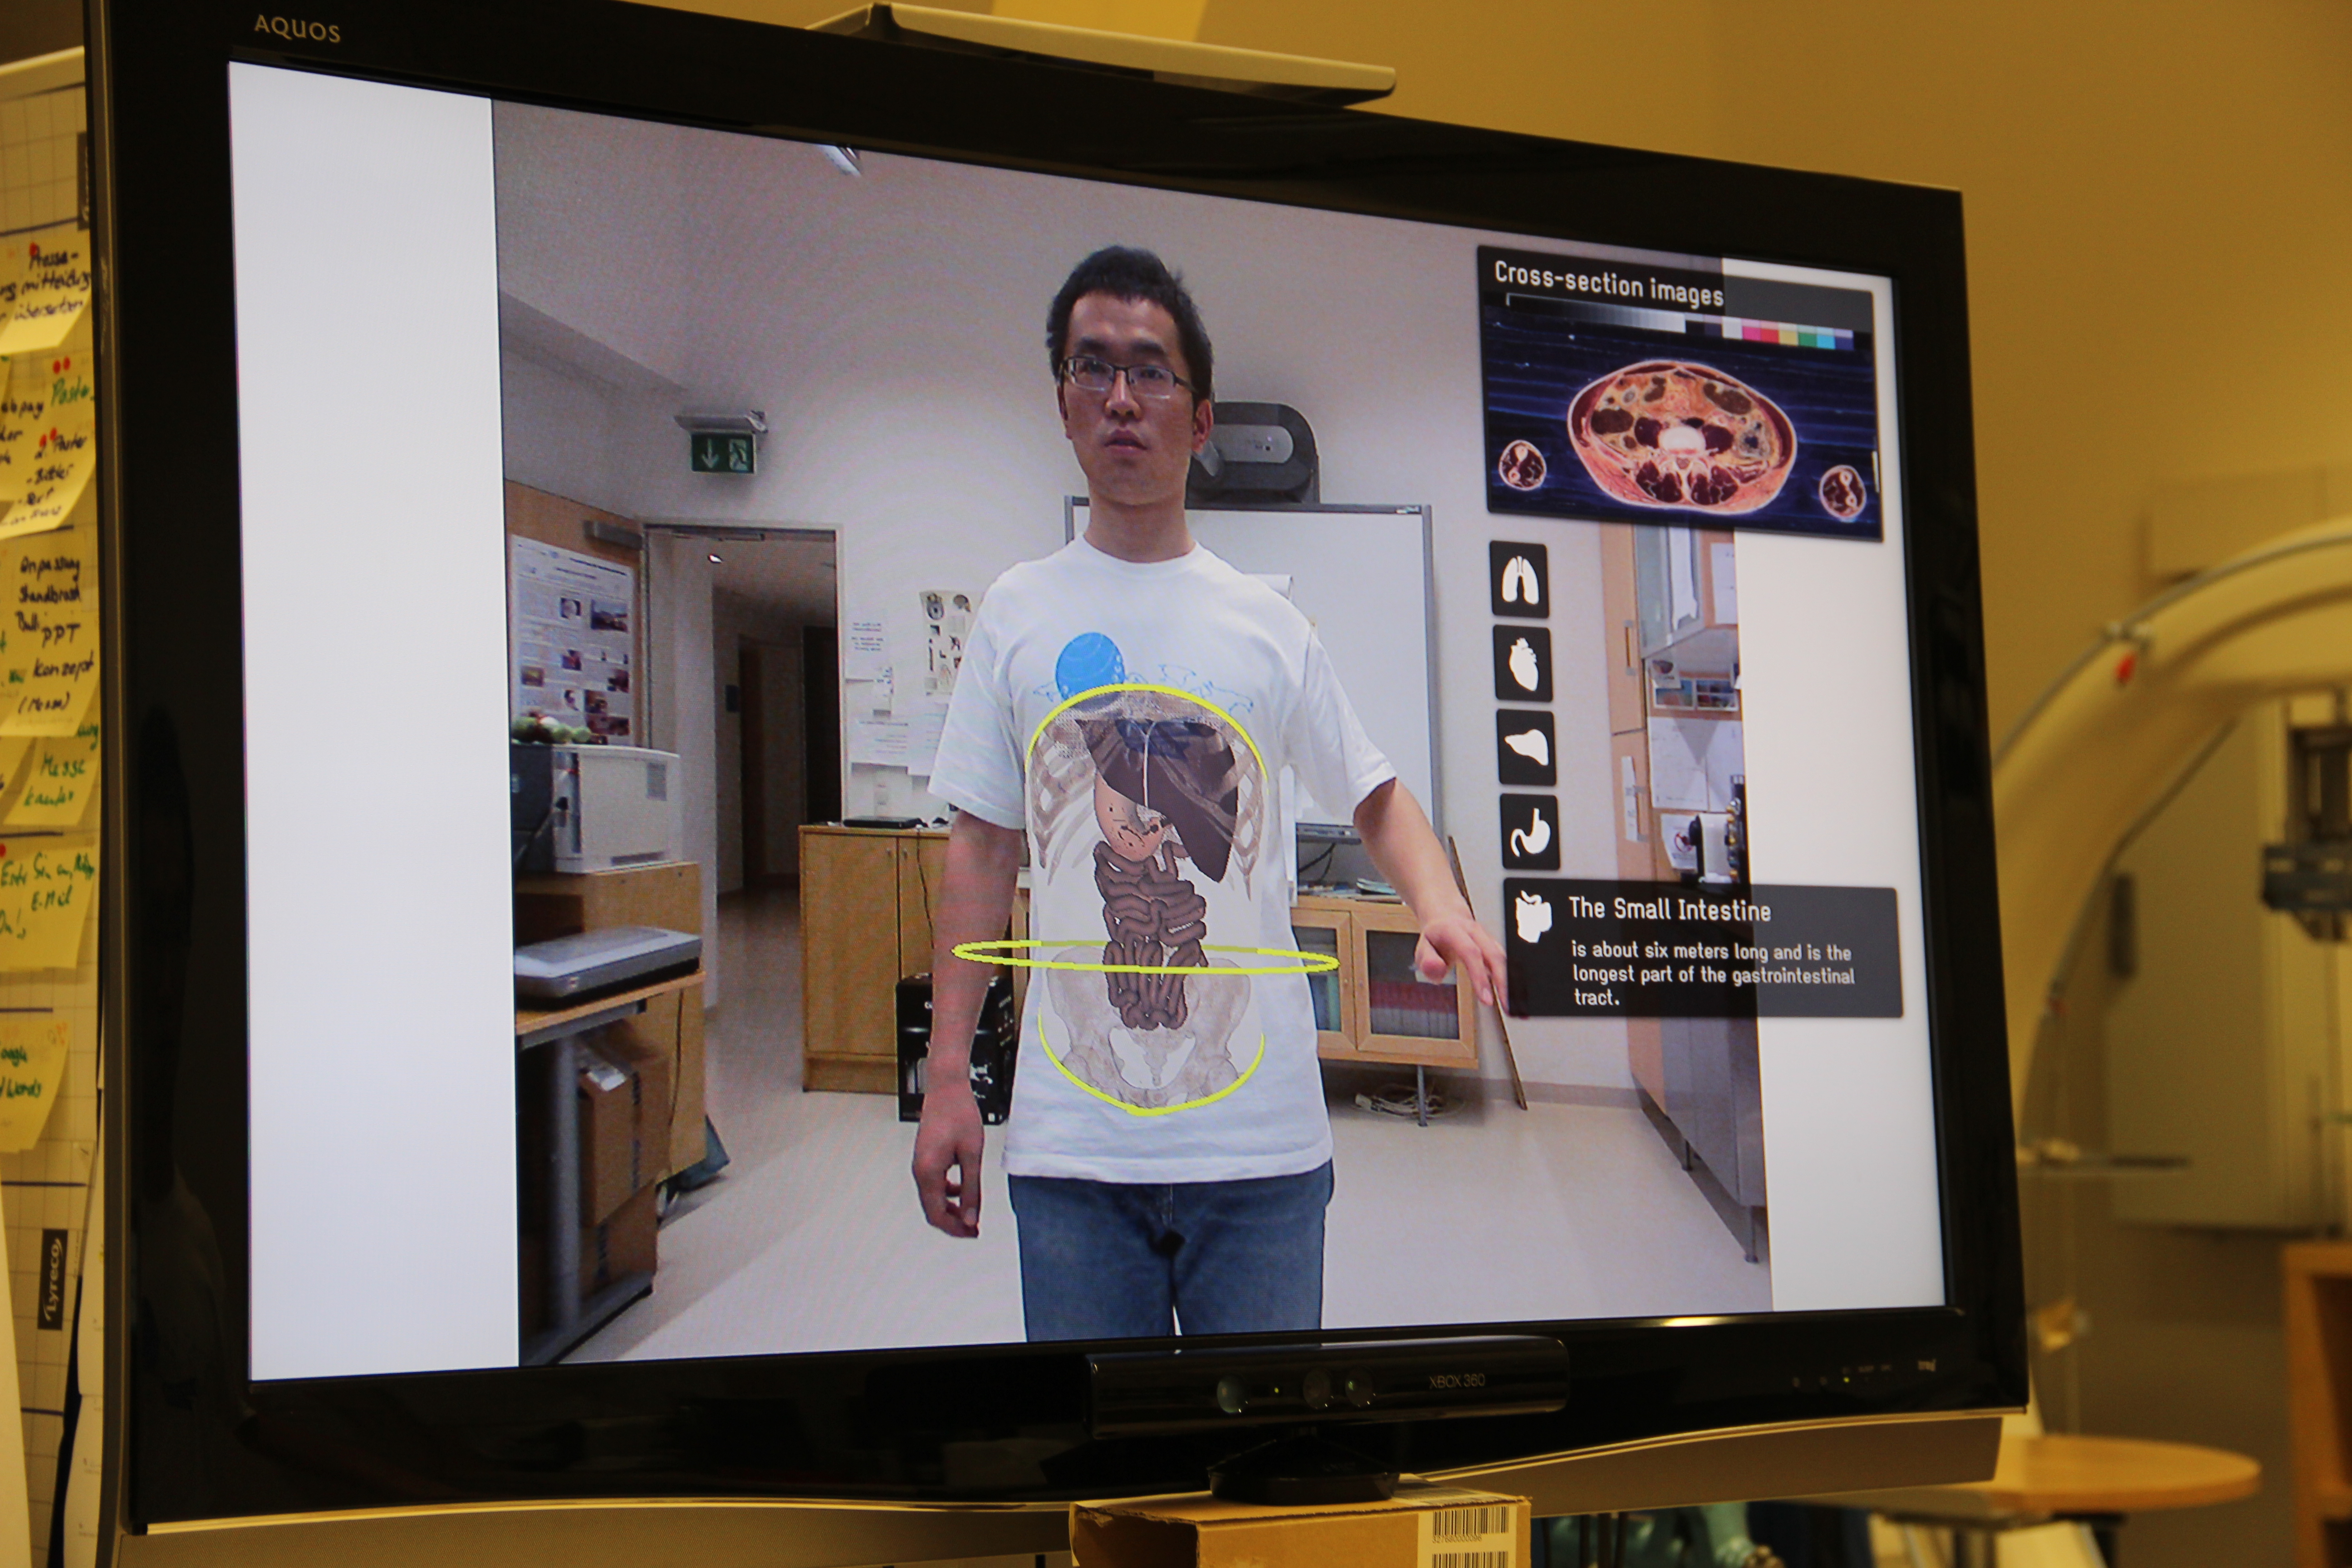
\includegraphics[width = 0.7\linewidth]{figures/3-MMC/Figure1.JPG}
	\label{fig:3-MMC:fingure1}
	\caption{Personalized magic mirror system for anatomy learning. A sensor tracks the user positions in real-time, and contextual in-situ visualization algorithms enable the augmentation of organs and muscles directly onto the user body.}
\end{figure}

\subsection{Natural perception and interaction}
\subsubsection{AR in-situ visualization of human anatomy}
For a personalized visualization of organs we employ the concept of a magic mirror. The camera image is flipped horizontally and shown on the screen such that the user has the impression of standing in front of a mirror. The system tracks all user movements using a depth camera and an algorithm to detect the pose of the user from the depth image. This is realized using the Microsoft Kinect which was originally developed to allow controlling computer games by motion. Then, virtual objects can be added to the image of the real scene. By using the magic mirror metaphor, the user is led to believe that he or she is able to look inside their own body. At the same time, radiological information (CT data and a fully segmented dataset of cross-sectional photographs of the human body) are displayed in real-time \cite{Blum2012}.

Prior to correctly using our AR magic mirror system, the users stand in front of the monitor and we displayed virtual marks near the five bone landmarks. The users are asked to interactively adjust the positions of the five marks to fit their own bone positions. In addition, the exact locations in the VKH CT dataset of the five selected bone landmarks are known. A linear interpolation was executed to estimate the torso point (i.e. a 6th landmark) in the CT volume to improve the overlay. Then the scale factors and transformation matrix were computed to render the anatomical image onto the user’s body. These landmark positions allow the deformation and interpolation of the medical data correctly within the magic mirror and onto the human body, resulting in a more precise augmentation. A user study involving surgeons and anatomy experts confirmed our findings and will be presented in Section 3.
\subsubsection{Natural User interaction}

\subsection{Potential application with magic mirror}
Medical education 
AR rehabilitation 
Patient positioning 

%todo: {Accuracy of Registration} improve the perception of the MR view via accurate registration. Anatomy learning, personal information (gender, age, body shape)
\section{Personal Registration of Magic Mirror}

\subsection{Personal Information}
We augment a personalized visualization of a CT dataset onto the user. However as full CT scans of any user are generally not available, we use the Visible Korean Human dataset (VKH), which consists of a CT scan, an MR volume and a photographic volume which has been acquired by stacking up cry sections. To allow a correct augmentation of the CT data, the gender, age, body size and pose of the user has to be detected. This is performed based on the color image using the OpenBR library \cite{Klontz2013} and the depth image using the NITE skeleton tracking software. The corresponding CT volume is chosen and scaled to the size of the user and augmented onto the user body. For visualization of the bones a transfer function is used as bones can be distinguished easily in the CT volume based on their voxel intensities. For the organs a segmentation of the VKH is used. The augmentation uses contextual in-situ visualization such that the virtual objects are only shown through a circular window. This leads to a better perception of depth, compared to a simple augmentation of the whole CT. The user could naturally turn around their body to check CT volume from different viewpoints and put their right hand at different heights to select a body plane with corresponding anatomy.

\subsection{Personal Registration}
We presents a general method to interactively improve and correct the Kinect skeleton for anatomy education purposes. We believe that our general method can be applied to projectors or other sensors as well for augmented reality. A thorough validation of our method demonstrated improved precision of anatomical landmarks and opens the avenue to future improvements in medical education. Together with the ISMAR community, we hope to initiate such discussions in integrating exciting user-interaction and gaming concepts within our system.

Our AR magic mirror relies on Kinect sensor which offers an imprecise skeleton tracking output (see \figurename{\ref{fig:3-PRMM:bonelandmarker}}). This limits the precision of our magic mirror augmentations offering users false anatomical positions overlaid onto their body, resulting in a poor medical learning environment. Alternatively, had we considered projectors to display human anatomy directly on a user’s body the same inaccuracies would exist\cite{Sun2013}. 
\begin{figure}[htb]
	\centering
	\label{fig:3-PRMM:bonelandmarker}
	\includegraphics[width = 0.75\linewidth]{figures/3-PRMM/FiveBoneLandmarker.png}
	\caption{Selected anatomical points for Kinect skeleton improvement and subsequent CT warping and interpolation.}
\end{figure}

The goal of this method is to propose a more precise user-specific learning environment. Together with orthopedic surgeons we have defined anatomical bone landmarks: (i) which are correctly identified in medical data such as CT and (ii) which users can touch easily on their body while standing in front of any sensor. These landmark positions allow the deformation and interpolation of the medical data correctly within the magic mirror and onto the human body, resulting in a more precise Kinect skeleton and augmentation. A user study involving surgeons and anatomy experts confirm our findings. 

The skeleton output from Kinect limits the precision of the AR magic mirror applications. Thus, our magic mirror augmentations would contain errors and users would easily distinguish anatomical offsets on their body resulting in a poor anatomy learning environment. Alternatively, we had considered projectors to display human anatomy and along with their existing limitations the same inaccuracies would exist. Our aim was then to propose a method to correct for such overlay inaccuracies that could be translated to any magic mirror system worldwide. Together with orthopedic surgeons, we have defined five bone landmarks that (i) users can easily identify and touch while standing in front of the Kinect, and (ii) that are accurately and easily identified in medical data such as CT \cite{ma2013ismar}. These are: left and right acromion, left and right anterior superior iliac spine, and the manubrium (see \figurename{\ref{fig:3-PRMM:5points}}).


\begin{figure}
	\centering
	\subfloat[~Improvement of Kinect skeleton]{
		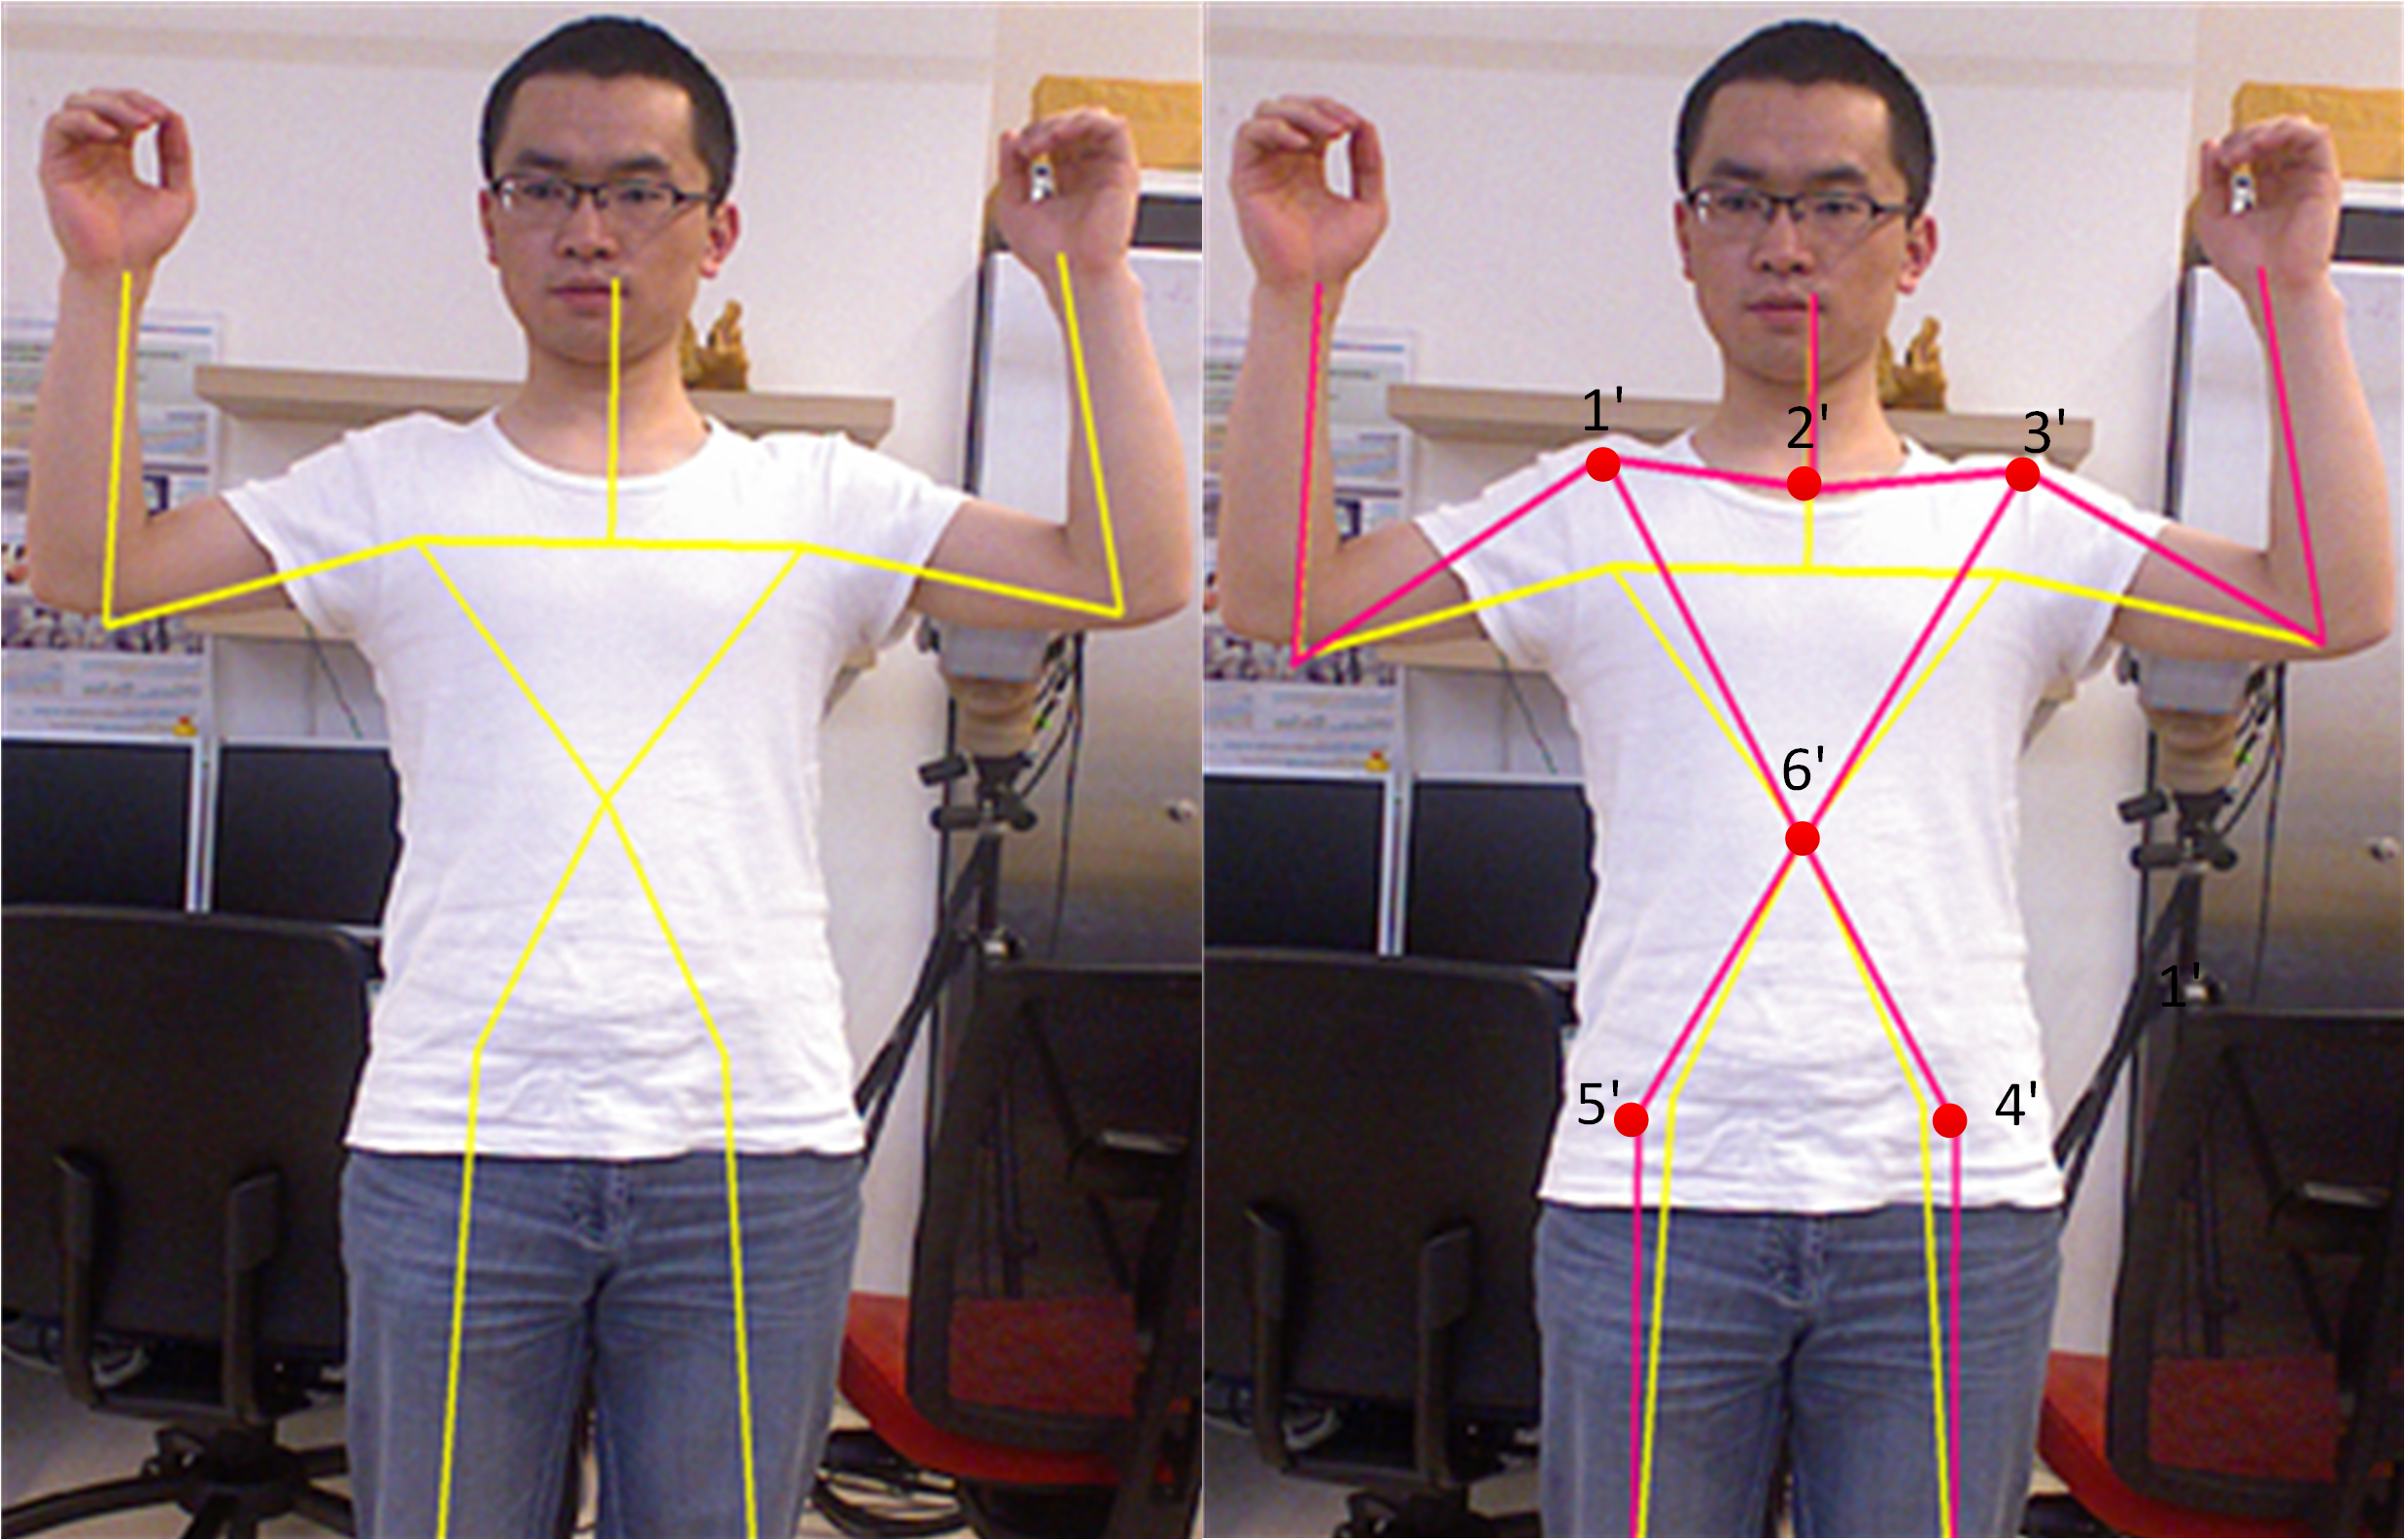
\includegraphics[height = 7cm]{figures/3-PRMM/ModifiedSkeleton.png}
		}
	\quad
	\subfloat[~Bone landmarker in CT volume]{
		\includegraphics[height = 7cm]{figures/3-PRMM/BoneLandmarkerInCT.png}
			}
	\label{fig:3-PRMM:5points}
	\caption{(a-b) The inaccurate Kinect skeleton, in yellow, compared to the improved Kinect skeleton positions in red. (c) CT data from the Visible Human Korean showing the 5 landmarks from Kinect skeleton. (d) CT data showing correctly the 5 landmarks + interpolated torso landmark using our method.}
\end{figure} 
\subsubsection{Anatomical bone landmarkers}
Together with orthopedic surgeons, we have defined five bone landmarks that can easily be touched on the human body. These are: left and right acromion, left and right anterior superior iliac spine, and the manubrium. Subjects are positioned in front of the Kinect sensor and asked to interactively adjust the positions of five landmarks
\subsubsection{Improment of kinect skeleton}
Figure 3 shows a comparison between the traditional Kinect skeleton and its proposed improvement. The first row depicts visually the exactness of the new skeleton. The second row depicts the skeleton landmarks directly on CT data. We observe that the shoulder and anterior superior spine are inaccurate in the images. The last row depicts the improved landmark positions within CT as well. Transverse and sagittal CT slices of the visible human Korean are seen respectively in rows 2 and 3.
In Figure 3a, the following scale factors were computed for the magic mirror augmentation:

\subsubsection{Evaluation}
As an augmented reality anatomy learning application, both accuracy and system usability are very important prior to its translation in classroom. Firstly, we undertook one user study with particular users having expert anatomy knowledge to evaluate if this system is precise enough for anatomy learning. Secondly, another user study involving first year medical students took place to verify the learning potential and acceptability of our technology as a compliment to atlas textbooks in classroom.

\paragraph{Assessing the magic mirror system precision and usability}
Participants: Seven participants were included in this study (two surgeons and five final year undergraduate medical students). 
Analysis: a Likert scale was used which is a type of psychometric response scale often used in surveys and the most widely used scale in survey research. When responding to a Likert questionnaire item, respondents specify their level of agreement to a statement. The format of our 5-pt Likert was: (1) strongly disagree, (2) disagree, (3) neither agree nor disagree, (4) agree, (5) strongly agree. 
To assess the precision of our personalized magic mirror we asked the participants to interact with the system platform which integrates user-specific anatomical landmark selection. Participants were asked to provide an estimated numerical offset, if any, on how far specific bone landmarks or organs were with respect to their own body. For this, they interacted with the magic mirror window, CT data, and used their own medical knowledge and expertise for judgment. CT data was displayed in an interface depicting both transverse and sagittal planes, and participants would quantify the offsets. If needed, a ruler was provided to assist them. The anatomical targets during evaluation were defined as: the anterior superior iliac spine, manubrium, heart, and liver. Results from this exercise are shown in \tablename{\ref{tb:3-PRMM:results1}}, with offsets measured in centimeters. Results from the user study show that the precision of user-specific learning environment is on average 0.96cm.
\begin{table}
	\caption{Precision (in cm) of magic mirror system based on anatomical offsets}
	\label{tb:3-PRMM:results1}
	\scriptsize
	\begin{center}
		\begin{tabular}{p{4cm}|p{3cm}}
			Anatomy & Offset(Mean$\pm$ STDev) \\
			\hline
			anterior superior iliac spine & $0.67\pm0.52$\\
			manubrium & $0.67\pm0.75$ \\
			heart & $1.17\pm1.60$\\
			liver & $1.33\pm1.21$
		\end{tabular}
	\end{center}
\end{table}

The seven participants were then asked to judge the usability of the AR magic mirror system by responding to the following questions: (i) is the overlay accurate w.r.t human body (ii) is the user interface easy to use, (iii) is it fun to play, (iv) can it be used for medical education, and (v) would it have stronger impact for medical education learning?
The Likert scale results for the first four questions are shown in \tablename{tb:3-PRMM:results2}.
\begin{table}
	\caption{Likert scale results regarding magic mirror usability}
	\label{tb:3-PRMM:results2}
	\scriptsize
	\begin{center}
		\begin{tabular}{p{6cm}|p{3cm}}
			\space & Mean$\pm$ STDev \\
			\hline
			is the augmented reality overlay accurate w.r.t human body & $4.00\pm0.89$\\
			is the user interface easy to use & $3.67\pm1.03$ \\
			is it fun to play & $4.50\pm0.55$\\
			can it be used for medical education & $4.17\pm0.75$
		\end{tabular}
	\end{center}
\end{table}
For the last question regarding the impact of our technology, there was a unanimous response that the AR magic mirror system should be considered as a potential platform to complement existing anatomy learning tools inside anatomy classrooms. 
\subsubsection{Discussion}
The precision of our method is visually demonstrated in Figure 3c-d and \figurename{\ref{fig:3-PRMM:ResComparing}}. We observe that the acromion and anterior superior iliac spine, using the traditional Kinect skeleton, is not positioned correctly within the CT data compared to the modified Kinect skeleton version (1-2 vs. 1'-2'; 3-4 vs. 3'-4'). The orthopedic surgeons participating in our study confirmed this.
\begin{figure}
	\centering
	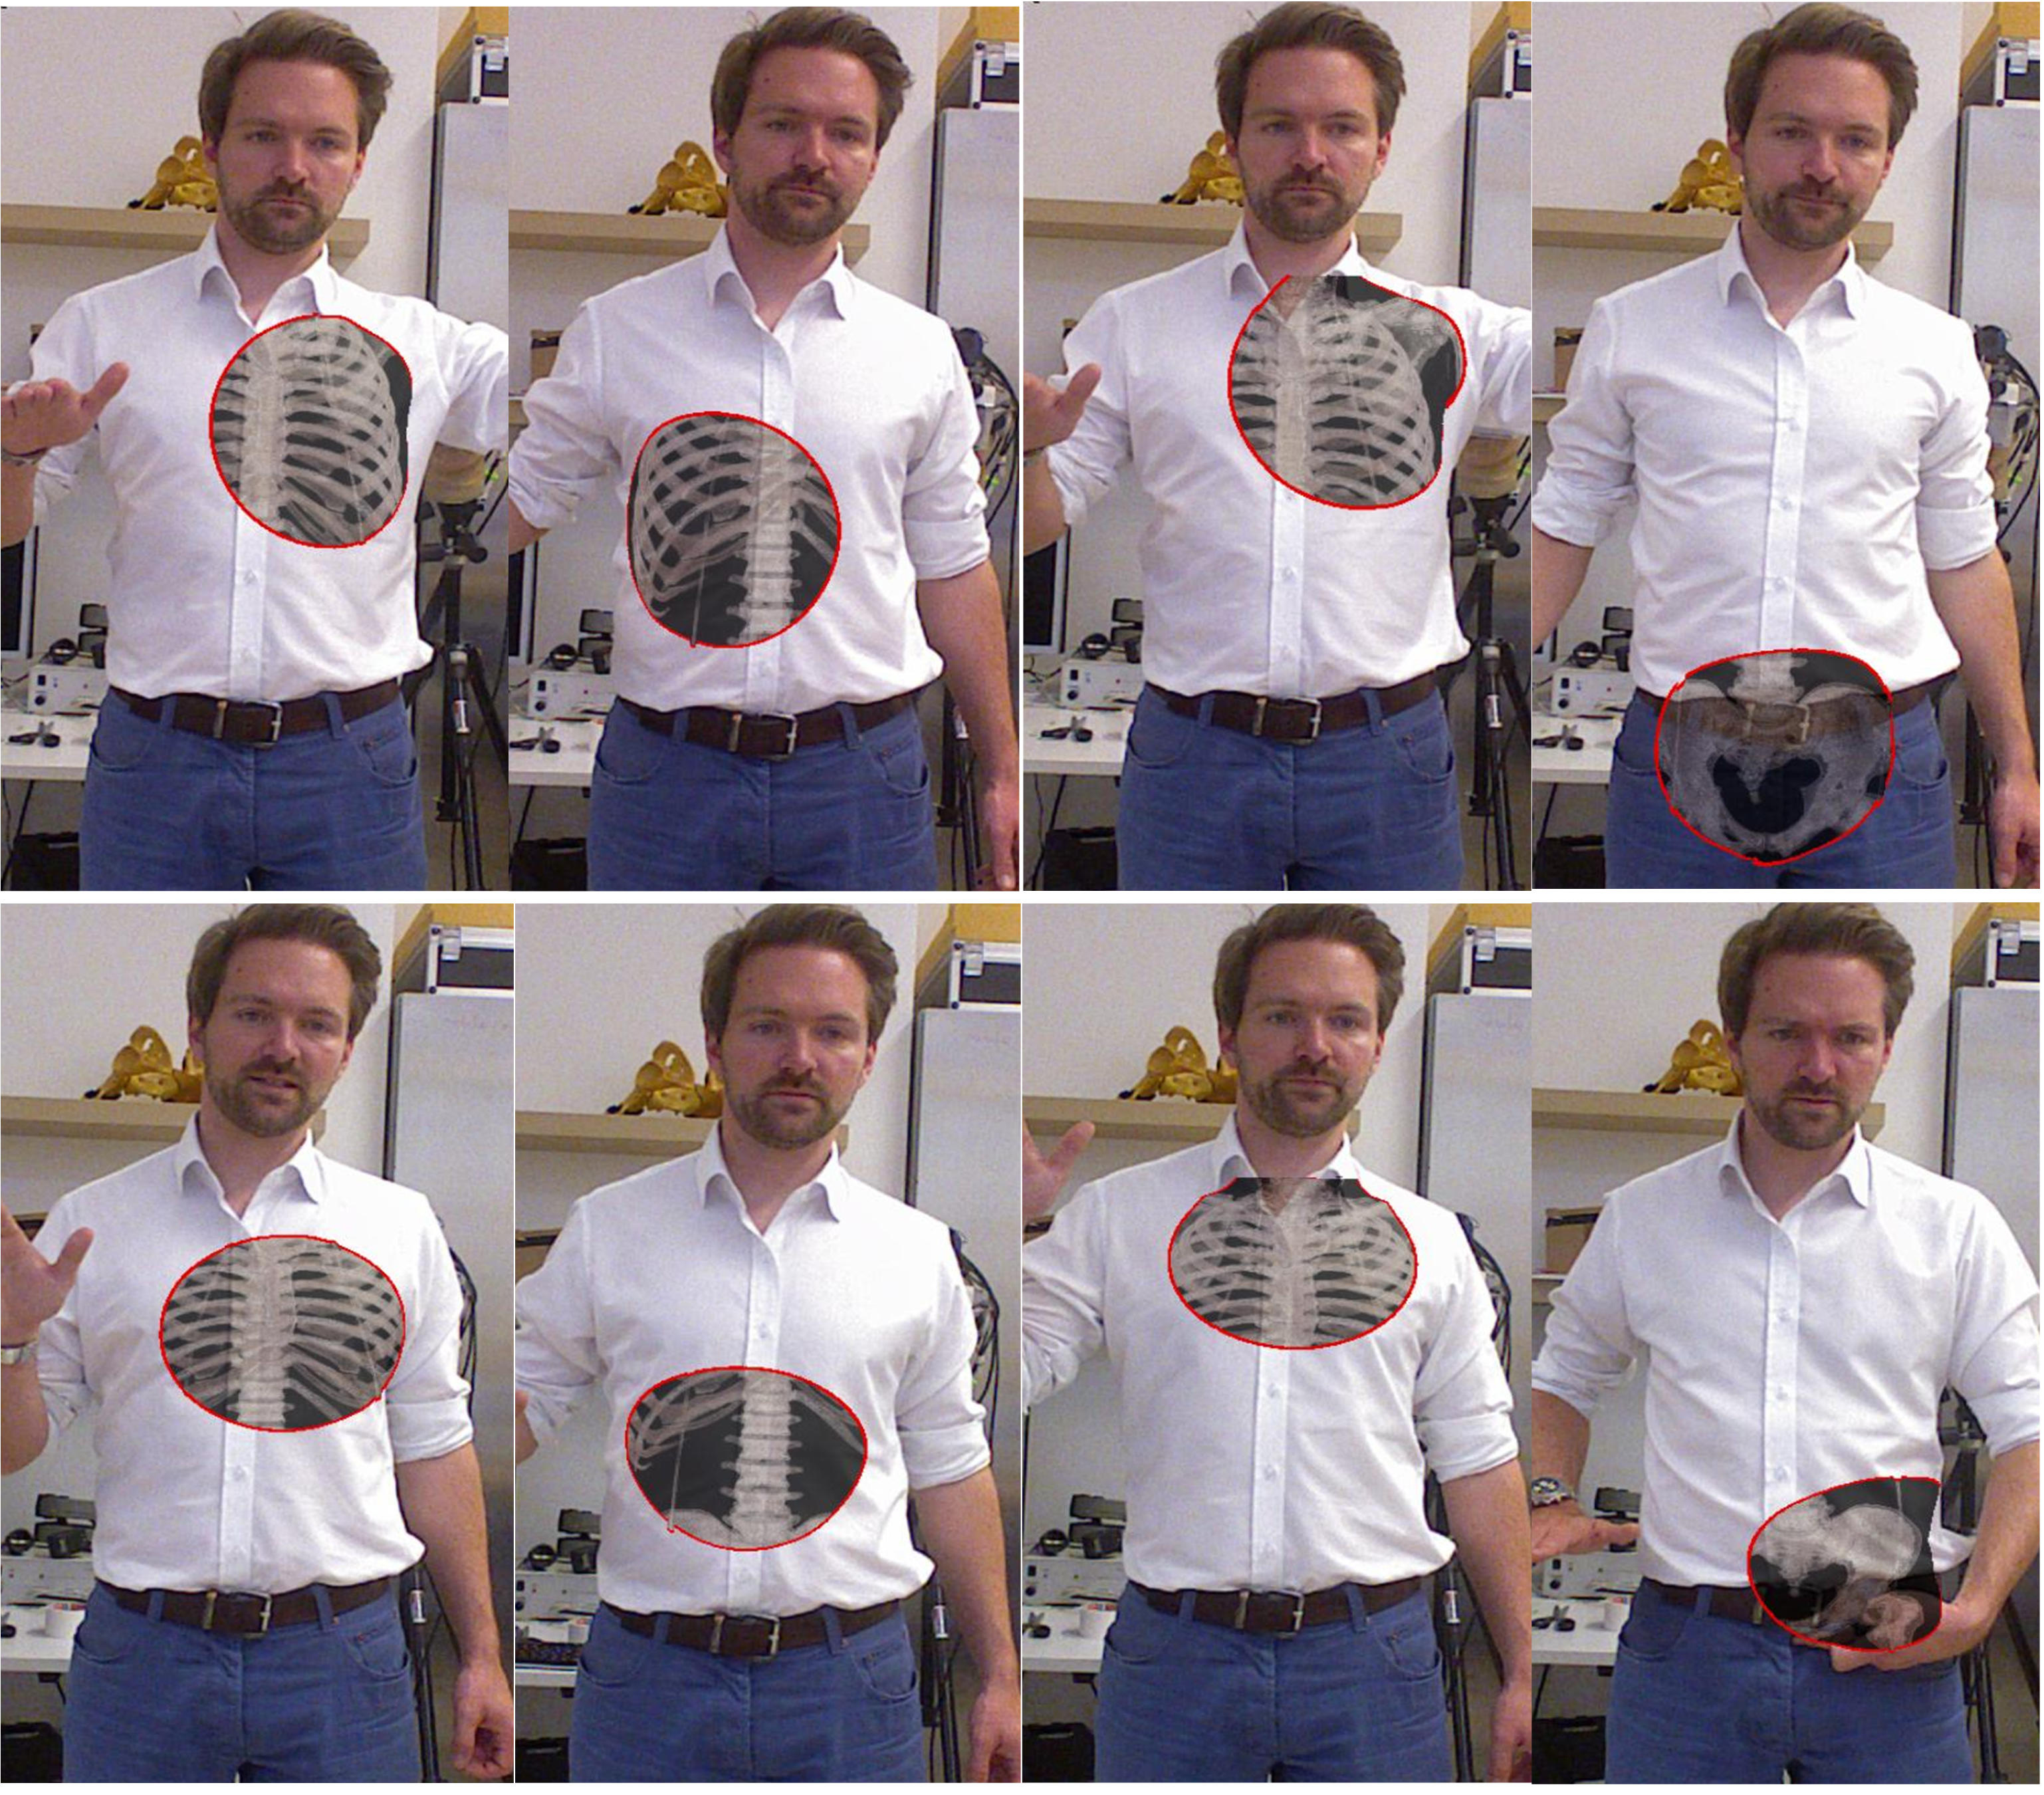
\includegraphics[width = \linewidth]{figures/3-PRMM/ResComparing.png}
	\label{fig:3-PRMM:ResComparing}
	\caption{Figure 4:	The magic mirror before (top) and after (bottom) the Kinect skeleton adjustment. Column 2 depicts the bottom of the rib cage being positioned correctly after skeleton correction.}
\end{figure}
Results from a user study show the impact of interactively improving the Kinect skeleton to increase precision for a better visualization of anatomy. The offsets of specific anatomical landmarks decreased significantly. The following comments were collected:
\begin{enumerate}
	\item the precision improved; making the user touch anatomical landmarks is cool since this is the way it is done in clinic…
	\item two additional landmarks easily accessible are the sternum and bottom of rib cage…
	\item make the magic mirror circle bigger for larger anatomy…
	\item voice command is a good idea but it is sensitive to the surroundings voice
	\item interactions between observers …
	\item could introduce the female CT visible human Korean…
	\item could use a healthy patient CT or other modality…
	\item could make the CT slices bigger on the screen…
\end{enumerate}

One appealing feature of the system is that with the Kinect we are using inexpensive standard hardware. In the future such a system could be made available to students or patients who have to do rehabilitation exercises at home. In addition to the full system using a large screen and a screen stand we also want to evaluate the benefit of making the system accessible to students when they are at home and at any time. We want to do this for two different reasons. First, there is a trend toward competency-based education in medicine. Instead of defining a curriculum, learning outcomes are defined. Students have to fulfill these learning outcomes. The advantage of competency-based education is that all students will have the same competency in the end. A student who is less skilled has to take more time to learn than a student who already has good skills. One requirement for this is that the students have to be able to educate themselves until they reach the required competency. We plan to use the AR magic mirror system both to allow them to do training and to test whether a learning outcome has been met. The magic mirror has to be made easily available to them so that they can use it for training at any time. The second reason to develop a distributed system which can easily be used by students is to collect user statistics.

Many medical education systems are web-based and allow accessing them from every computer. However current systems do not use high-end visualization and input devices like the Kinect. In the future when technologies like HTML5 and WebGL have matured it can be imagined that a system like the magic mirror could be implemented using web technology such that it can run on any computer. However, at the moment the use of web technology would be a significant limitation. We are using very large datasets, high-end visualization, GPU computing and gesture-based interaction.

It was originally suggested to us that our system would have much more of an impact for medical education learning if it were to be translated today in medical schools and anatomy classrooms. As such, with the help of our co-author and anatomy professor, we deliver the improved AR magic mirror to two anatomy classes within the Anatomy Department of the Ludwig Maximilian University (LMU) Medical School, Munich, Germany. The anatomy professors made it clear that the AR magic mirror system is exciting, but has to go beyond state-of-the-art technology to be truly useful for education. Our participants stressed the importance of visualization of anatomy that can change dynamically resulting from the actions of the user moving the body, and also for visualization of muscles. Furthermore, more advanced user interactions like the use of gaming elements would be required to make the use of the system for learning tasks more interesting.
% !TEX root = ../thesis-example.tex

%todo: Make the user believe the virtual element is a part of his or her own body. (Organ game and the Muscle learning)
\section{Interactive Mixed Reality and Serious Gaming} \label{sec:3-PPMM:IMR}
%Personalized natural interaction \& gaming
Although we can lean by reading and watching and real depth of understanding, the learner always needs to encode the knowledge herself, rather than simply receive what is shown. This is one of the reasons that interacting with the mixed reality system can be a powerful learning tool - we are not only get the benefit of AR view, but also receiving immediate feedback. Knowledge is a process of understanding by connecting. These interactions are often useful in creating the aha moment -- the joining of medical knowledge with a learner's own body and movement.
In last section, user's personal information was collected to improve the general perception of the medical information.
Here, we tried to implement several applications in integrating exciting user-interaction and gaming concepts within the proposed magic mirror framework.
 
%Two kinds: user motivate interaction (user's movement trigger the changing) and scenario interaction (AR view change according to the presetting), combine two kinds together. 
The basic magic mirror system focuses on the abdomen organs as real-time deformation of the 3D medical images is very difficult. Firstly, we extent the magic mirror to visualize the basic function of the human skeleton and muscle system, since each bone of the skeleton system is also a rigid object and is controlled by muscles via attachment points. Besides mirroring the users movements to the skeleton, the system  also visualizes active muscles and implement a labeling system, which can be used to show the names of the muscles or bones.
Then, a new interaction with anatomy is developed for learning in the augmented reality magic mirror framework. It allows the implementation of independent modules on top of mirracle, which is demonstrated by the two modules for the organ atlas and the education game that are already taking advantage of this infrastructure. The organ atlas is a good way of imparting anatomical knowledge on the users, allowing them to explore their body without any instructor or supervisor.
The interaction methods we developed are not necessarily limited to self-referenced selection and manipulation. In general cases, they are suitable for scenarios where many possible items are densely packed and a user wants to select a single or multiple items in an augmented or mixed reality environment. The large number of possible modifications to the methods make them difficult to configure, but the general ideas should be applicable to many use cases.
Thirdly, Figure 4 depicts the visualization of muscle anatomy of a human arm. The magic mirror was embraced by the majority of the medical students in its current version. Based on our discussion with them we found that the students really liked the AR visualization on their own bodies, however they were not used to the natural user interface and gestures required for interaction. A learning curve was necessary for them to appease initial frustrations they had when first using our system.
Finally, serious gaming for education and rehabilitation is discussed. One education game is developed taking advantage of the new interaction method with the anatomy, and a AR knee rehabilitation demo is developed. 

\subsection{musculoskeletal Animation} \label{sec:3-IMR:musculoskeletal}
Instead of rendering the bones from a rigid CT dataset, a polygonal model will be used to create the AR view of the skeleton. Then, we can animate the model based on the orientation of the joints received from the skeleton stream to match the pose of the user in front of the system.
The objective of this application is to develop a simple non-physical visual effect of the musculoskeletal system based on models from OpenSim\footnote{\url{https://simtk.org/home/opensim}}, which is freely available, user extensible software system that lets users develop models of musculoskeletal structures and create dynamic simulations of movement. Besides mirroring the users movements to the skeleton, the system also visualizes the relationship between bones and muscles. Furthermore, a labeling system is implemented which can be used to teach the user names of the muscles or bones (see \figurename{\ref{fig:3-IMR:skeletonMuscleDemo}}).

\begin{figure}
	\centering
	\includegraphics[width=0.7\linewidth]{figures/3-IMR/skeleton_Muscle2.png}
	\caption{Musculoskeletal Animation in magic mirror: an application to show a simple non-physical visual effect of the musculoskeletal system based on models from OpenSim}
	\label{fig:3-IMR:skeletonMuscleDemo}
\end{figure}

\subsubsection{OpenSim Musculoskeletal Model}
OpenSim is an open source software platform for biomechanical modeling, simulation, and analysis. The GUI includes many tools for loading data, creating and editing models, visualization of the simulation results, and much more. The API allows programmers to access the core components of OpenSim to create new plug-ins for the GUI or take advantage from it in theirs own applications. It also includes some validated musculoskeletal models and more can be downloaded from the platform website\footnote{\url{www.simtk.org}} where researchers can provide their work \cite{Delp2007}.

OpenSim Musculoskeletal Models consist of bodies, joints, forces, constraints, controllers, markers, and contact geometry (see \figurename{\ref{fig:3-IMR:openSimModel}}). The skeleton is build up with rigid bodies and joints connecting two bodies. A body has attributes for its mass, center of mass, and inertia. It can include display geometry for bones. Joints have an attribute for their position in the parent body and hold a joint type dependent transformation to define the motion of a body relative to its parent body. Movements can be further restricted by constraints. Muscles are modeled as forces that are exerted on attachment points to the rigid bodies. The force of the muscle is dependent on its path (through all the attachment points) and muscle properties like maximum force, optimal fiber length, tendon slack length, pennation angle, and maximum contraction velocity. 
From the OpenSim models, we can definitely use the skeleton model and the paths of the muscles, by a conversion of the geometry data and reorganization of the scene graph. But, the muscle states simulation functions are difficult to integrate into magic mirror system, since it can not calculate the muscle activity in real time.
\begin{figure}
	\centering
	\includegraphics[width=0.8\linewidth]{figures/3-IMR/openSimModel.png}
	\caption{OpenSim Musculoskeletal Model: The skeleton is build up with rigid bodies and joints connecting two bodies. Muscles are modeled as forces that are exerted on attachment points to the rigid bodies. }
	\label{fig:3-IMR:openSimModel}
\end{figure}

\subsubsection{Application Design}
Based on the magic mirror framework, the application is designed according to the following rules. The objective is a simple interactive MR application for education.
\begin{itemize}
	\item Accurate AR view of the skeleton.
	\item Clear relationship between the bones and muscles.
	\item Estimate the muscle active states when the user performs movements.
	\item Highlight the active muscle according to the movements.
	\item Information of the bones and muscles for learning.
\end{itemize}
A general musculoskeletal model is created according to the OpenSim models and it contains the bone geometry, connections between the bones, muscles and attachment points to the bones. Skeleton and muscles are load to the application as two separated sub scene graphs, as  the skeleton model can be used independently for many purposes. In real world, the muscles control the bone movements, but the muscle model is dependent of the skeleton model in the application as the system input are just the positions and orientations of the skeleton joints. The skeleton model is transformed based on the skeleton stream from the Kinect and the muscle model is then updated as it is affixed on the bones via the attachment points. Both models are rendered to create the non-physical visual effect to generate the AR view. 

\paragraph{Update Skeleton Model}
After a user is calibrated, the skeleton model is scaled to fit the current body. The proportion of the user can be estimated through the pose matrices. The scale method first scales the root node which is the pelvis and it actually scales the whole model. 
The scale factor is calculated from the distance of the right shoulder to the left hip. So this scale factors represents the average of width and height of the torso relative to the general model. In practice using this approximation gave better results then calculating two different scale factors. 
The accuracy of the proportions of the legs could be improved by calculating the distances between hip, knee, and ankle. We employ the same scale as the torso when the knees and ankles are not observed by the sensor.
Here we also define a calibration pose to get an accurate measurement of the segment length. 
The calculation of the transformation of each joint on the model is also another important task. The relationship between the coordinates spaces of Kinect, OpenGL, and the skeleton model has to be carefully analyzed. In order to obtain the correct relative rotation of each bone, quite a few transformations have to be apply to the raw joint orientation from skeleton stream. The skeleton model is then animated to mirror the body movements.

\paragraph{Update Muscle model}
The muscle model contains all the individual muscles, which is displayed in the application. Each muscle is model as a 3D string which goes through all the attachment points. So the muscle model is dependent of the skeleton model and is first created based on the general skeleton model. Wherever the skeleton model is updated, each muscle model is also recreated to make sure the size and special relationship is correct. 

%add an attachment point to define the path of each muscle model 
The attachment point information for each muscle is textually found inside the OpenSim 'osim' model file. Each attachment point is defined by the bone's name, 3D position in the bone coordinate system, and the type of point. One muscle has several attachment points, which define the relationship with the bones. A xml file is create to save all muscle information.
In the application, 3D strings are rendered between each pair adjacent attachment points. 
The color of the string is defined as the active state of the muscle and the line width can be adjust according to the muscle's size. The muscle model is not hierarchical as the skeleton model. Muscles are attached to bones in different coordinate systems. As the attachment point is defined in the bone coordinate system, the positions have to be converted to the world space. The world position of the bone is easily calculated by accumulating all the transformations from the skeleton root to the current bone object. Then, each attachment point can be converted to the world space.

A Label class is designed to show text information of the bones and muscles. The Label is meant to display text attached by an arrow to a point in the scene. The special feature of this class is that two labels will never overlap. The originating point of each label is from the object, e.g., a bone or a muscle, and where the text is actually drawn depends on the sorted vector of the all visible labels. The text is drawn always below the text of the label previous and connected with a line to the originating point (see \figurename{\ref{fig:3-IMR:openSimModel}}).

%update muscle color 
When a new frame comes in, the system updates the skeleton model according to the orientation of the each joint. And the world coordinates of each bone and attachment points are calculated. The length of each muscle can be estimated by the distances between the points. The active state of the muscle can be simple assessed based on the length change. A muscle is active when its lengths is shorter than the initial length or at least shorter than its previous length.  In this case the color will be scaled between red and green dependent on the difference. Red means that the muscle is active and green means that the muscle is approximately inactive. It depends on the contraction speed and the length of the muscle. This method does not compute forces like OpenSim, it only estimates the activeness of the muscle very coarsely. Finally, muscles are redrawn with the new position and new color.

OpenSim provides some advanced function to simulate the active states of the each muscle based on the body movement, but the approximation in real time is not possible right now and only the skeleton position stream is too noisy for such simulation. Another possible solution to fetch more accurate muscle state is to attach electromyographic sensors onto the user's body. This should be one of the future work for this thesis. 
%In the next step the color of the muscle is recalculated.
%The color is going have a portion of green of intensity and a portion of blue of 1-intensity. The intensity is defined as the square difference of the length and previous length of the muscle normalize by the initial length. So the intensity is influenced by the speed of the contraction. If the length of the muscle is shorter than the initial length then one can average it with intensity2 for the actual amount of contraction to simulate gravity.The formula for intensity  is obtained experimentally.
%If the muscle is active this is calculation of the color:
%\begin{figure}
%\centering
%\includegraphics[width=0.7\linewidth]{figures/3-IMR/mulcleActiveColor}
%\caption{To calculate the muscle active state and the color mapping function}
%\label{fig:3-IMP:mulcleActiveColor}
%\end{figure}

\subsection{Interaction for Anatomy Learning} \label{sec:3-IMR:anatomyLearning}
Basic Knowledge of human anatomy is not only important for medical doctors or health-care professionals, it is also considered common knowledge that is taught at various levels of school education. To improve the conventional book-based methods for anatomical education, we investigate the suitability of an augmented reality system using a magic mirror metaphor for this task.
With the existing platform serving as a basis, we first have developed an abstraction framework offering a general interaction for augmented-reality applications. On top of this framework, we have implemented an interactive educational application consisting of an organ atlas and a complementary organ learning game, leveraging the benefits of self-referential learning and motivation through game challenges.
%To achieve intuitive usability, we investigate different user interaction methods for organ selection in a self-referential system using augmented reality, providing methods for unique selection as well as coarse, non-unique selection.
\paragraph{Interaction Challenge}
The most challenging problem of the idea turned out to be the selection and interaction methods with the organ model. For our idea to work, we need a method to reliably detect which organ the user has selected while leveraging the mirror analogy as far as possible. The most intuitive and direct way would be to use a virtual hand technique to directly select the organs \cite{Ha2010}. This, however, is bound to fail for two reasons:
First and most obviously, it is not possible for the user to put his hand into his body and directly touch the organ, he is merely able to point to the approximate region in front of the organ. This region he is able to indicate is not accurate and in many cases it is not really possible to detect reliably which organ the user meant. Especially in the abdominal area many organs are fit very tightly together in one place, making it very hard to distinguish between two organs.
Secondly, the tracking capabilities of the current version of Kinect sensor used in our implementation are somewhat limited. The only thing suitable for selection that is reliably tracked is the position of the hands. Neither orientation of the hand nor information about the fingers is available. This makes it even harder to develop a suitable, intuitive interface. Untrained users usually use their fingers when asked to indicate a point, but since we can only track the hand position, there is always an offset to our tracked position and the position the user was actually indicating, and this offset is not static but depends on the hand orientation and size and position of the fingers we know nothing about.

\subsubsection{Motivation and Objective}
To provide an alternative method for medical teaching, we have developed a computer-based system allowing the users to have a virtual look into their body. We use the magic mirror concept as a basis for our augmented reality application: The users can see themselves on the screen like in a mirror, but with additional information like computer models of their inner organs augmented onto his body. Here, we try to expand this existing implementation to be used as an alternative and entertaining way to teach human anatomy. A general framework to support generic extensions of the magic mirror system is first implemented. Using this framework, we implement an educational application, an interactive organ atlas to allow the user to explore his body and learn about spatial relations, visual appearance and function of the organs. An organ learning game to provide an entertaining way to learn anatomy is also presented in section \ref{sec:3-IMR:gaming}. This game is based on the knowledge presented in the atlas and leverages augmented reality and motivation through game challenges to improve the learning performance of the user. To achieve this goal, we examine different interaction metaphors and their suitability for the tasks presented.

In the AR learning environment, organ selection is a challenging task as some organs hide behind others. The user cannot directly position their hand into their bodies and to select the organ of choice. In engineering design, mechanical parts are drawn with the innermost part at the center, while the others are moved some fixed distance outwards to display all parts of the assembly that would otherwise be hidden. Inspired by this principle we designed and developed an organ explosion effect (see \figurename{\ref{fig:3-IMR:organExplosion}} ), which separates the organs. The organ explosion selection employs a two-hand interaction method. Using the left hand, the user is able to focus the height for the section they are interested in. Organs at approximately the same height are then projected outwards. Using a spherical projection, the organs are moved outward, creating the illusion of seeing them `fly out' in front of the body. Lines are drawn to indicate the original position of the organs. After separating the organs from each other, it is easy for the user to select the organ of interest using their right hand. Another functionality of the organ explosion effect is allowing the user to rotate and observe the 3D organ models and perceive the spatial relationship between them.

We implement an interactive anatomy atlas that is, in our first prototype, limited to the inner organs of the torso. The user can explore these organs and read additional information on each of the visualized organs. The work is separated into two different parts: A general framework performing all kinds of basic operations not specific to any application and the actual application logic implementation and realizing the organ atlas application.
The general interaction framework is designed to be an abstraction layer on the magic mirror framework and provides easy access to implement custom application logic, making it easier to experiment with new ideas based on the magic mirror system.

\subsubsection{System framework}
The main design goal is that abstraction is extensibility, to encapsulate all the interaction and visualization functions behind the application logic layer. Hence,  it is very easy to implement new games and other applications or experiments using the offered interaction interface.
The requirement is the possibility to develop different applications based on the framework and allowing integrating them into one single application with as little effort as possible. 

The investigation of possible interaction methods forms an important part of this work. Since conventional point-and-click selection methods are only of limited use for self-referential selection in AR environments, we have developed new methods better suited for our use case: One is driven by a two-handed interaction method to allow the user to select the region of interest with one hand and using the other hand to select a specific organ; The other uses a single-handed approach where the user indicates the organ directly by touching the specific region of his anterior torso. The system then detects possible selections and thus does not provide a single, unique selection in most cases.

\paragraph{organ Explosion}
Our approach to overcome the selection challenge is a technique that we, have called ``Organ Explosion" effect (see \figurename{\ref{fig:3-IMR:organExplosion}}). This technique is inspired by exploded view drawings known from engineering, where the goal is to depict how mechanical parts are to be assembled. Usually they are drawn with the innermost part at the center while the other parts are moved some fixed distance outwards to display all parts of the assembly that would otherwise be hidden.
We use the same basic idea in our interaction technique by implementing a two-handed interaction method: Using the left hand, the user is able to set the focus height for the region he is interested in. Organs at approximately the same height are then projected outwards. Because we use a spherical projection with the center at the height of the hand, but at a point behind the body, the organs are moved outwards, creating the illusion of seeing them fly in front of the body. This way we are able to separate the organs close together since organs at different angles to the projection point are projected into different regions. We scale the magnitude of the displacement down with the distance between hand and body to allow the user to see the organs in their original arrangement but still enable him to ``zoom in" for detail and selection. \figurename{\ref{fig:3-IMR:organExplosion:b}} depicts how this technique looks in practice.
Once we are able to separate the organs from each other, it is easy to check for selections using a direct mapping from the physical right hand to the virtual one and just checking for intersections between the hand and the organs.
\begin{figure}
	\caption[Organ Explosion]{Left: Quantities involved in the calculation of the position offsets for the technique (organs not displayed). In this image, four organs are displaced. Purple dots are original organ positions, blue dots displaced organ positions. The Yellow dot signifies the projection center. Right: Screenshot of the explosion technique.}
	\label{fig:3-IMR:organExplosion}
	\subfloat[Front View] {\label{fig:3-IMR:organExplosion:a} 
		\includegraphics[height= 7cm]{figures/3-IMR/organExplosion2}}
	\subfloat[Side View] {\label{fig:3-IMR:organExplosion:b} 
		\includegraphics[height= 7cm]{figures/3-IMR/organExplosion1}}
\end{figure}

\paragraph{Interaction test for Selection}
Intersection detection between different 3D objects is a built-in functionality in rendering library. A virtual predefined sphere or cylinder is attached to control hand of the current user. The selection function is triggered when the intersection test between the hand object and the organ models. 
For performance reasons, we only use bounding-box intersection tests and skip the narrow phase, treating intersecting bounding-boxes as intersections between geometry. This obviously reduces the accuracy of bounding box tests, this coarse intersection check is better not only in performance, but also from a usability perspective. Intersection tests in our applications are used for checking intersections of the hands with organs. Due to the inaccurate tracking of the hands by Kinect, this actually works quite good when just checking for ``roughly" intersecting pairs.

To further improve performance, we introduce an explicit vector that describes objects that are actually interested in intersections with other objects. The assumption is that general intersections, for example between two organs, are not of interest, while intersections with special objects like a sphere attached to the user's hand are interesting and important.
Once an ``interesting" intersection has been determined between a pair of objects, the first object gets added to the intersecting objects list of the second and vice-versa. This list can then be used and analyzed in the behavior implementation to perform reactions to the collisions.
For convenience reasons, there are two vectors configured to be attached to the left and right hand. They can be added to the framework if required and reconfigured by the application implementation.

\subsubsection{Organ Atlas Application} spatial ralationship and 3D information of the model 
An organ atlas is usually a collection of visual representations of organs or specific organ systems, annotated with names and further information.
We tried to reproduce a version of this concept using our magic mirror framework to implement this idea interactive. The main educational goal of this application is to allow the user to explore the organs of his body and learn about the position, function and spatial relations to the other organs.
We approach this goal by augmenting all available organs onto the user's body and letting him select the one he is interested in. Once the user has selected an organ, the application displays textual information about the organ. This information includes the common, latin and/or greek names as well as a description of the basic purpose of the organ. During the selection procedure, the spatial knowledge of this organ is also learned. If applicable, the organ system it belongs to is mentioned as well as the principle organs it interacts with. An example of what the application looks like in action and finished is shown in \figurename{\ref{fig:3-IMR:OrganAtlas}}.
\begin{figure}
\centering
\subfloat [In action] {\label{fig:3-IMR:OrganAtlas:a} 
	\includegraphics[width = 0.5\linewidth]{figures/3-IMR/FrontViewOrganExplosion}}
\subfloat [Finished] {\label{fig:3-IMR:OrganAtlas:b} 
	\includegraphics[width = 0.5\linewidth]{figures/3-IMR/OrganAtlas}}
\caption{Organ Atlas implementation. Lungs are selected and the infobox shows textbook knowledge about them.}
\label{fig:3-IMR:OrganAtlas}
\end{figure}

The organ atlas described above together with the described exploration and optimized selection methods, offers an interesting new way to explore the human anatomy. However, the described methods offer much room for experiments and improvement. The optimal choice of all parameter values is a very delicate matter that has not been explored fully in this work. The values chosen on an empirical basis seem ``good enough" to at least show that the methods work reasonably well to be used productively. To determine a better parameter, one should conduct a separate study and compare the performance results to generate the parameter settings according to the personal information of the untrained users. Also, the different variations of the methods offer even more room for fine-tuning the effectiveness of this method. 
The organ learning game in its current prototype version already provides a fun experience, but it lacks the content to be distributed as a full game. This could easily be changed by adding more game modes for other organ systems, multi-player modes or other elements commonly found in games.
 
\subsection{Interactive Muscle learning}
Muscles is one very important and difficult topic for all the medical students (see \figurename{\ref{fig:3-IMR:armAnatomy}}). The visual details of the muscle is not presented in the section \ref{sec:3-IMR:musculoskeletal} and functions of the muscle is not easy to learned from the static atlas.  
To evaluate the learning effect of magic mirror, another application framework is developed for muscle learning, currently focusing on the main muscles of one arm related to four basic movements, \textit{flexion}, \textit{extension}, \textit{pronation}, and \textit{supination}. 
The learning targets are the main muscles, which expand and contract during the above movements (see \tablename{\ref{tb:3-IMR:motionMuscles}}).
\begin{figure}
	\centering
	\subfloat{
		\includegraphics[width=0.35\linewidth]{figures/3-IMR/armAnatomy1}
	}
	\subfloat{
		\includegraphics[width=0.35\linewidth]{figures/3-IMR/armAnatomy2}
	}
	\caption{Anatomy of the arm}
	\label{fig:3-IMR:armAnatomy}
\end{figure}
\begin{table}
	\caption[Muscles involved]{The selected motion of one arm and the corresponding muscles}
	\centering
	\label{tb:3-IMR:motionMuscles}
	\scriptsize
	\begin{center}
		\begin{tabular}{|c|c|}
			\hline
			Motion & Muscles \\
			\hline
			\multirow{2}{*}{Flexion} & M.biceps brachii \\
			& M.brachialis \\
			\hline
			\multirow{2}{*}{Extension} & M.triceps brachii \\
			& M.anconeus \\
			\hline
			\multirow{2}{*}{Pronation} & M.pronator teres \\
			& M.pronator quadratus \\
			\hline
			Supination &M.supinator \\
			\hline
		\end{tabular}
	\end{center}
\end{table}

\paragraph{Motivation}
The main objective of the application is to enable the user to acquire knowledge about the bones and muscles of the arm, connecting the procedure with their own arm movement. Based on the magic mirror framework, the non-physical visual effect is the activities of the muscles and the bones. A virtual model of an arm is rendered according to the real arm movement and the AR view is generated.

\paragraph{Application Design}
The application should contain an AR view, which shows the complete color image from the Kinect with the augmented virtual arm. This view acts as the mirror effect and help the user to map all the activities of the bones and muscles onto his/her own arm. Aside from this AR view, there is another virtual view which is program controlled. The virtual view concentrates on the upper or lower arm, showing the details of the muscle model. To preserve the connection between the user and the virtual arm, the AR-view is shown on the left side of the screen after the user is calibrated. The arm model in virtual view only follows the relevant motions, i.e. flexion, extension, pronation and supination. 
The learning patterns include muscle oriented, muscle is displayed one by one, and motion oriented, the user performs the target motions and only the muscles related the current motion is shown. 
We also have to make sure the user can observe the muscle model from different view to learn the spatial information and the learning flow is smooth and friendly. 

\subsubsection{Dynamical muscle model}
\paragraph{Skeleton information}
The position and rotation of the skeleton model are defined in a strict hierarchical order, starting with the spine. The position data from Kinect skeleton stream is in the world coordinate system. To animate the arm model, the relative orientations have to be calculated based on the position of the joints. Only the spine position is directly set as the root's position in the AR view. 
The lower arm is treated separately to the other bone chains. Each hand's orientation is defined using the vectors from the wrist to the tip of the hand, and from the wrist to the thumb. Additionally, to be able to follow the shoulder's full range of movement, the upper arm uses the direction of the lower arm to define its orientation along its length axis.
In order to adjust to differences in the users' height and physique, the individual bones are scaled whenever a new user is selected. For each node, the distance between its position and the position of the next node in the chain is used to calculate the scaling factor. To increase the accuracy, that distance is averaged over multiple frames before calculating the scaling.
%That makes it possible to use the absolute rotations from the Kinect with a hierarchical skeleton that would usually prefer relative orientations. With hierarchical skeletons, the position data from Kinect is only used for nodes without parent, the remaining nodes are positioned through their parent's rotation and scaling, thus only the root's position is set directly in a complete skeleton. This behavior can be disabled to always use the absolute positions even with hierarchical skeletons. As with the positions, there are two modes to rotate the nodes to choose from. The first one uses the rotation from Kinect, modified according to the axis-settings in the skeleton. The second uses the position data to calculate the orientation via Look-Rotation to align one axis with a \textit{lookAt-target}. To define the orientation along this look-direction, a second vector is supplied. Unity offers a function to create a Look-Rotation, but this always aligns the objects z-axis with the target and uses its local y-axis to define the axial rotation, so a more flexible version of this function was implemented.
%\begin{figure}
%\centering
%\includegraphics[width=0.7\linewidth]{figures/3-IMR/LookingRotation}
%\caption{Look-Rotation along the object's local x-axis (red)}
%\label{fig:3-IMR:LookingRotation}
%\end{figure}
\paragraph{Muscles and Bones}
An anatomical model of a human male body from ANATOMIUM 3D\footnote{\url{http://www.anatomium.com/}} is employed as the virtual arm model. This model includes all the anatomy, such as skin, muscles, bones, blood vessels and so on (see \figurename{\ref{fig:3-IMR:humanModel}}).
\begin{figure}[htb]
	\centering
	\subfloat[Skin]{\label{fig:3-IMR:humanModel:a}
		\includegraphics[width=0.32\linewidth]{figures/3-IMR/muscleSkin}}
	\subfloat[Muscles]{\label{fig:3-IMR:humanModel:b}
		\includegraphics[width=0.32\linewidth]{figures/3-IMR/muscleMuscles}}
	\subfloat[Skeleton]{\label{fig:3-IMR:humanModel:c}
		\includegraphics[width=0.32\linewidth]{figures/3-IMR/muscleSkeleton}}
	\caption{Anatomy model from ANATOMIUM 3D}
	\label{fig:3-IMR:humanModel}
\end{figure}

Since the application only covers just one arm and quite a few simple motions, this muscle and skeleton model was simplified under the supervision of a senior medical student. Only the bones of the arm and the shoulder, and the muscles responsible for the motions, flexion, extension, pronation, and supination, are included, i.e. the \textit{musculus biceps brachii, musculus triceps brachii, musculus brachialis, musculus anconeus, musculus pronator teres, musculus pronator quadratus and musculus supinator}. The \textit{musculus coracobrachialis} was added to this collection according to the medical partner's suggestion, although it does not contribute to the motions mentioned above.

The bone models are used as they were, but after consulting with medical professionals, we decided to recreate the muscle models, since the existing ones did not resemble their real counterparts closely enough. The biceps and triceps were present as two respectively three separate parts, and the position of the anchor points of most muscles did not correspond to their real-world position. To achieve a more realistic visual effect, the muscle model should be deformed during the selected motions.
The texture of the 3D muscle model is realistic, especially in a close up view. It is quite difficult to apply vertex weights to the mesh topology of the original muscle model. 
Most muscles were modeled with a cylindrical base mesh that was modified using polygonal modeling techniques and subdivision algorithms according to images from the Sobotta Atlas of Human Anatomy (see \figurename{\ref{fig:3-IMR:modifiedArmModel}}). Only the supinator and the pronator quadratus where modeled from a flat box, due to their shape. The biceps and triceps were both created as one contiguous model instead of separate parts for each head and detailed attention was given to the anchor points for all muscles to make sure they are at the correct positions.
\begin{figure}[htb]
	\centering
	\subfloat[Flexors]{\label{fig:3-IMR:modifiedArmModel:a}
		\includegraphics[width=0.32\linewidth]{figures/3-IMR/muscleFlexor1}
		\includegraphics[width=0.32\linewidth]{figures/3-IMR/muscleFlexor2}
		}
	\quad
	\subfloat[Extersors]{\label{fig:3-IMR:modifiedArmModel:b}
		\includegraphics[width=0.32\linewidth]{figures/3-IMR/muscleExternsor}}
	\subfloat[Pronators]{\label{fig:3-IMR:modifiedArmModel:c}
		\includegraphics[width=0.32\linewidth]{figures/3-IMR/musclePronators}}
	\subfloat[Supinator]{\label{fig:3-IMR:modifiedArmModel:d}
		\includegraphics[width=0.32\linewidth]{figures/3-IMR/muscleSupinator}}
	\caption{Dynamic Muscle Models}
	\label{fig:3-IMR:modifiedArmModel}
\end{figure}

%todo review the following paragraph later.
To enable the animation of the arm model, the bones are weighted to an armature that consists of one control object for each the upper and lower arm and the hand. In order for the ulna and radius to behave correctly when the hand is rotated, they are weighted to separate control objects. These are parented to the control object for the upper arm to define their position, but their orientation is controlled by a LookAt-Constraint to rotate them towards a helper object parented to the control object for the hand.
To deform the muscles, the vertices of each model are weighted to several control objects, which can be transformed easily. The vertices follow the transformation of each related object to a special percentage, which is determined by their weighting. When these virtual muscles are scaled non-uniformly, meaning they get thinner when they elongate and vice versa, the muscle meshes react to this scaling, and since each vertex has slightly different weights, the mesh deforms, resembling a real working muscle. Each of the control object is itself controlled by two helper objects that define the muscles anchor points and are parented to the appropriate bones.
\begin{figure}[htb]
	\centering
	\subfloat[Arm Model]{\label{fig:3-IMR:modelArmature:a}
		\includegraphics[width=0.32\linewidth]{figures/3-IMR/ArmatureMuscle}}
	\subfloat[Armature]{\label{fig:3-IMR:modelArmature:b}
		\includegraphics[width=0.32\linewidth]{figures/3-IMR/Armature}}
	\subfloat[Armature with Muscles]{\label{fig:3-IMR:modelArmature:c}
		\includegraphics[width=0.32\linewidth]{figures/3-IMR/ArmatureWithMuscle}}
	\caption{Dynamic Muscle Models}
	\label{fig:3-IMR:modelArmature}
\end{figure}
The muscles' animation for contraction and expansion was achieved in 3ds max via stretchy bones, which automatically contract or expand, if their length is changed. Furthermore, since the muscles have to correctly react to the user's movement, creating fixed animation that can be played in the engine would not have been feasible. This was accomplished by a configuring class attached to each muscle's control object. It contains references to the control object's two anchor points and uses them to define its position and rotation. The position is set directly to that of the first anchor, while the rotation is calculated via a relative rotation. To control the expansion and contraction of the muscles, it measures the distance between the control object's anchor points and scales it along its local x-axis according to the ratio between that distance and its neutral length. Along the y- and z-axis the inverse of that ratio is used for scaling, multiplied by a factor to control the magnitude of expansion. Whenever a new user is selected, the neutral length of each muscle is recalculated after the skeleton is scaled.

\subsubsection{Learning Functionality}
\paragraph{Virtual view}
The details of the muscle is very important topic, so virtual view is introduced to present a close up view of the arm model. There are several solutions to place the virtual camera. One is that the camera rotates around a special object and generate the virtual view from different angles. The cameras are each parented to a rotating helper object to create an orbiting movement around the arms. 
%Additionally, it can be influenced by the user in order to have an even closer look at areas of interest. In all views, the active muscles are highlighted.
The close views are implemented with additional cameras and copies of the arm model. By putting these copies into separate layers it is ensured that these cameras only render their respective arm. The models are not directly controlled by the user through a Skeleton Manager, but instead imitate the movement of the original arm along single axes only. This way, the first copy takes part in just the flexion and extension, while the second one participates in the pronation and supination. The muscles not responsible for the respective movement were removed, to keep them from obscuring the relevant muscles or distract from them.
\begin{figure}
	\centering
	\subfloat[View 1]{ \label{fig:3-IMR:MuscleLearningVirtualCamera:a}
		\includegraphics[width=0.47\linewidth]{figures/3-IMR/MuscleLearningVirtualCamera}}
	\subfloat[View 2]{ \label{fig:3-IMR:MuscleLearningVirtualCamera:b}
		\includegraphics[width=0.47\linewidth]{figures/3-IMR/MuscleVirtualCamera}}
	
	\caption{Virtual Camera concentrating on Flexion and Extension}
	\label{fig:3-IMR:MuscleLearningVirtualCamera}
\end{figure}

\paragraph{Self-control virtual view}
We also introduce a self-control virtual camera, whose position and rotation can be controlled by the user. When the user's right hand is placed close to the left arm, the self-control camera model is triggered. The camera moves to the position of the hand and tries to focus on the desired area by calculating the closest point on the arm and rotating towards it (see \figurename{\ref{fig:3-IMR:selfControlCamera}}). This point is computed in the user-controlled arm's local coordinate system and transformed into that of the arm currently observed. As shown in \figurename{\ref{fig:3-IMR:MuscleLearningSelfControlCamera}}, the user can naturally move the virtual camera to focus on different objects from different view angle. This function introduces more friendly interaction for learning.
\begin{figure} [htb]
\centering
\includegraphics[width=0.5\linewidth]{figures/3-IMR/selfControlCamera}
\caption{The camera moves to the position of the hand and tries to focus on the desired area by calculating the closest point on the arm and rotating towards it}
\label{fig:3-IMR:selfControlCamera}
\end{figure}

\begin{figure}
	\centering
	\includegraphics[width=0.7\linewidth]{figures/3-IMR/MuscleLearningSelfControlCamera}
	\caption{When the user's right hand is placed close to the left arm, the self-control camera model is triggered.}
	\label{fig:3-IMR:MuscleLearningSelfControlCamera}
\end{figure}
\paragraph{Interactive learning}
A configuring class is defined, including methods to control the muscles' visibility, the highlighting of working muscles and of anchor points, and the labels that display the muscles' names and function. For highlighting it determines the angle between the upper and lower arm, as well as the rotation of the hand, relative to the frame before. This information is used to determine which motion is being performed, and in turn, according to \tablename{\ref{tb:3-IMR:motionMuscles}}, which muscles are active. 
In an earlier prototype, each muscle controlled the highlighting itself by measuring the change in length, but this data proved to be too inaccurate and produced noticeable flickering. The abstraction using only the angles between the joints of the arm yielded smoother results. Additional functions expose the ability to toggle the visibility of all muscle-labels to the User Interface and enable it to control the visibility of muscles by type.
Similar to the muscles, the bones are controlled by a configuring class. These determine the color-coding of the bones and expose this functionality to the UI and the learning sequence.
In muscle oriented model, one or one group muscle is shown successively and AR view and virtual view of the Muscle is generated. The user can perceive the detail of the muscle, the start and end point and the spatial relationship with the bone (see \figurename{\ref{fig:3-IMR:muscleModelLearning}}). In motion oriented model, user are asked to perform special arm movement and only the muscle involved is highlight (see \figurename{\ref{fig:3-IMR:MuscleLearningVirtualCamera:b}}). Then the functions of the muscle is learned. 
During the learning procedure, the user can always move the arm and see the muscle state and shape deformation.
When a motion is performed, active muscles would furthermore be visually highlighted in order to make them more prominent.
\begin{figure}
\centering
\includegraphics[width=0.7\linewidth]{figures/3-IMR/muscleModel}
\caption{muscle oriented model: one muscle is shown and the user can perceive the detail of the muscle, the start and end point and the spatial relationship with the bone.}
\label{fig:3-IMR:muscleModelLearning}
\end{figure}

\paragraph{Learning Sequence}
Based on the AR and Virtual view, the system can generate a lot of learning material. We prefer a simple user interface and let the user focus on the learning not  how to control this system. However, natural interaction would not introduce any barrier. Hence, we introduce another function, ``Learning Sequence".
The sequence of events for the learning session is defined via a configuring file. This an easily editable text format with values separated by semicolons. Each line in this file contains the data for one event. The data for one event consists of an integer for the duration and the camera mode, boolean values to enable or disable the color-coding for the bones, the muscles' labels and highlighting of their anchor points and a bitmask that determines the muscles visibility. Each bit in this eight-digit binary number controls visibility for one muscle. An optional seventh value can be used to display text at the bottom on the screen. 
This file is opened and read line by line by a simple parser at the start of the program, and the data is stored in an array of event structure. 
The sequence is played using a coroutine that takes one entry from the event-array and uses its values to set the relevant parameters and waits for the specified time before repeating this with the next event, until it reaches the end of the array. Simple functions can control the running sequence by stopping and restarting the coroutine or by modifying the array-index to skip or replay events.

To facilitate the learning session, the users run through a predefined sequence of events. It starts with the AR-view, showing the bones of the arm, identified by color, with the muscles hidden. It then switches to the first close view to introduce the muscles for flexion and extension individually. Next to each muscle with a label displaying its name and additional information about its function. After the muscles contributing to each motion have been introduced, they are shown together to give the user the opportunity to recap. This process is then repeated for pronation and supination using the second close view. 
The whole sequence runs for approximately ten minutes and can be stopped, paused or resumed at any time. Additionally, it is possible to skip events or return to passed ones. Both the color-coding and the labels showing the muscle-information can also be displayed independently from the learning sequence.

%\subsubsection{Evaluation}
%todo data from Ina's thesis
\subsubsection{conclusion}
The user study was conducted at various locations, with test subjects of different backgrounds. 
%The users were divided into two groups, the first of which used the application, while users from the second group were handed conventional materials, i.e. a section from an atlas of human anatomy, to learn the same information. Both groups got twenty minutes to acquire as much information about the arm as possible, which meant for those using the application to run through the sequence twice. 
After this time was up, each user was to fill out a questionnaire.
By the time of writing the results of the study was not yet analyzed, but from the witnessed sessions it became apparent that most students who tried the application viewed it as an interesting and engaging source of information. The possibility of viewing the arm from every direction offered them a new insight that they could not get from static images. This application is limited by necessity, so the textbook still constitutes a more universal resource, but it can function as a useful supplement. If the study confirms the effectiveness of acquiring knowledge with an AR-program, a further developed application could possibly include and convey a higher percentage of the information offered in the book, but the feasibility of replacing it completely seems debatable.

\subsection{Serious gaming} \label{sec:3-IMR:gaming}
%todo: maybe the subsection come first then the senction: interactive muscle learning
Rehabilitation and whacke an organ

Health education and rehabilitation is a particular area where serious gaming is suited \cite{Aubin2012,Jonas2012}. We developed a game for general users to learn basic anatomy called Whack an Organ (see Figure 3-right).

\subsubsection{Organ game}
Our game is based on the idea of the classic arcade games at carnivals, ‘Whack-a-Mole'. We implement a similar game idea using our application framework developed in section \ref{sec:3-IMR:anatomyLearning}. It is a combination of Whack-a-Mole and classical quiz games. Questions regarding human anatomy is shown to the user, and the answers are always one organ or organ system. This knowledge will serve as a basis for the interactive organ learning game. This game works in a quiz-show like manner where the user has to answer questions by indicating the right positions of the organs.
To answer the question, the user has to point to the location of the organ directly on their body. The game then decides if the location is correct and awards points if so. Questions can come from different question sets with varying difficulty, ranging from simple location questions: \textit{where is the liver?}, to more complex knowledge questions: \textit{which organ is infected if you have Hepatitis?}.
Still, the questions have to have a concrete organ as an answer, limiting the possible range of anatomy-related questions. At the end of a question round, the achieved points are shown to provide some feedback on the performance on the player.
We hope to provide an experience that is both entertaining and fun to persons of all ages, but due to the simplicity of the questions and detail of information displayed, for our first version, the target group can be considered children and teenagers where the common knowledge about human anatomy is not as present as with more adult persons.

\paragraph{Organ Selection}
When the user place his/her hand onto their body, the selection organ or organ system has to be detected to check if the answer is right. 
A direct approach is to do the bounding box interaction test between all the organ and the object, which is attached to the hand. 
Once an intersection has been detected, we again use a timeout to allow the user to position the hand correctly. Once the timeout has run out, we use all organs that are currently intersecting with the hand as our selection set (see \figurename{\ref{fig:3-IMR:organGamingBoundingBoxSelection:a}}).
Because we only use bounding box intersections, it seems obvious to use a simple box attached to the hands. We increase the length of the box in negative Z direction (towards the back of the body) to be as long as the torso is ``deep". This is because some organs like the kidneys are located in the dorsal area of the torso and they still have to intersect with the box when the player touches the front.

\begin{figure}[htb]
	\centering
	\subfloat[Bounding box]{ \label{fig:3-IMR:organGamingBoundingBoxSelection:a}
		\includegraphics[width=0.45\linewidth]{figures/3-IMR/organGamingBoundingBoxSelection}
		}
	\subfloat[Sphere interaction]{ \label{fig:3-IMR:organGamingBoundingBoxSelection:b}
		\includegraphics[width=0.45\linewidth]{figures/3-IMR/organGamingSphereSelection}
	}
	\caption{Debug visualization output of the two selection techniques. (a) Organ Bounding Box Selection: Blue box is intersector box of the left hand. (b) Sphere Selection: Blue spheres are the selection regions, red sphere is the intersector of the right hand}
	\label{fig:3-IMR:organGamingBoundingBoxSelection}
\end{figure}
\paragraph{Sphere intersection}
Another solution is inspired by taking the Whack-a-Mole concept one step further. We use a fixed number of selection regions attached to the body of the user. Those regions, implemented as virtual spheres, are attached to the front of the trunk and are separated far enough to allow for an unambiguous selection of one of the spheres using the hands. They act as a proxy for the actual organs, so the user only has to select the sphere closest to the organ in question.

We detect the selection of the spheres by using the hand positions of the player and calculating the intersections. It often happens that the hand passes through another selection area while the player moves the hand towards the desired position. We prevent erroneous selection through this effect by using a selection timeout. One sphere must be selected exclusively for a certain time to trigger the selection.
Once we have detected the selection, we have to determine if the user has chosen a correct answer. To check this, we precompute the closest sphere for every organ at the initialization. We then are able to check if the correct organ(s) are associated with the selected sphere and determine the correctness of the answer.
The number of spheres can be varied that are possible for selection. 
%Increasing the number of spheres has a number of effects on the method. At a first glance, the accuracy gets better: The more selection spheres there are, the closer an associated sphere is to the actual center of the organ. On the other hand, it gets considerably harder to select the correct sphere the smaller they get. Not only is it problematic when the sphere radius gets smaller than the organ size, but also the tracking stability of NiTE suffers when the user holds his hand in front of the body, resulting in selections the user didn't intend just because the skeleton tracking was wrong. Practical tests suggested that a grid of 3x3 or 3x4 spheres is the best choice for this method. 
Another modification would be to allow several spheres to be associated with an organ. This could solve the problems with tracking inaccuracy and also help increase the number of spheres. However, this requires a more sophisticated algorithm to determine which spheres are associated to which organs.
Finally, a more radical modification would be to only use one sphere/ellipsoid of the approximate size of the torso. This would only be used as a dummy to detect when the player has touched the body. Once this touch has been detected, we could determine the selection by including all organs at a certain radius from the hand in the selection set. 

\paragraph{Implementation}
The implementation of the game is rather straightforward based on the application framework. We first load an appropriate question set from the hard drive. Question sets consist of a list of questions together with a set of correct answers for each question. The answers are given as a list of organ names, and calculate the closest sphere if needed.
After setting up the basic game state variables like the current question and counters for correct/wrong answers, we proceed to set up a default behavior for all organs. This behavior keeps an organ invisible for most of the time. Only when the user has selected an answer and the organ is in the set of correct answers for the current question, it is made visible for a short time (see \figurename{\ref{fig:3-IMR:organGaming}}). At the time, it flashes either red or green, depending on whether the answer as right or wrong.
For the first selection method, we now set up the intersection spheres on a regular grid in body space. After we have determined the positions of the sphere centers, we perform the calculation for the nearest spheres for each organ. The spheres and the results of this calculation are stored as static variables to allow the hand behavior access to this data.
\begin{figure}
\centering
\includegraphics[width=0.7\linewidth]{figures/3-IMR/organGaming}
\caption{organ gaming}
\label{fig:3-IMR:organGaming}
\end{figure}
The behavior functions for left and right hand are identical in this game to allow the user to select answers with both hands.
For the sphere-based method we test the intersection between the hand object and spheres. In the behavior, we then determine whether the hand is currently intersecting a sphere and if so, decrease our timeout. If the timeout has run out, we determine the selection set by using all the associated organs of the selected sphere.
If we use the bounding box method, we just check if an intersection between hand object and organs has been detected to decrease our timeout. When it has timed out, we use all intersecting organs as the selection set.
Once we have determined a selection set, we continue to check whether it contains a correct answer. According to this, we play a short feedback sound and increase the counter for correct or wrong answers. Afterwards we check if there are any question left. If so, we just display the next question. One important thing for usability is to prevent the system from accepting the current position as an answer for the next question as well, because the hand is still intersecting and the timer has run out. We chose to solve this by setting a flag that prevents accepting new answers. This flag is only cleared when the user has moved the hand completely away from the body.

The organ learning game implemented as a proof of concept offers an engaging and fun way to learn about the human anatomy. The intuitive concept of indicating the organs on the players' own body should offer an increased learning intention. 
We hope to extend the system by providing different difficulty levels to make it more interesting for a larger target group.

\subsubsection{rehabilitation}
The Rehabilitation Game using Kinect for leg stability and balance training is a game aimed at patients that need to undergo rehabilitation of a leg or need to train balance because of an injury or due to great age. It is designed to monitor the patient during the rehabilitation exercise as well as entertain him while doing the exercise. The most important function for the application is the ability to track human bodies with the Kinect device. This functions is used to create an augmented reality environment and to track the stance of the player.
The Kinect device is used to achieve a greenscreen effect and transfer a video of the patient onto a screen in real time. The patient sees himself on a screen in a virtual environment and plays the game by moving his free limbs while balancing on one leg. The first goal of the programm is to use the Kinect to monitor the patient and to ensure that he is keeping the pose required for the rehabilitation exercise and his balance. The poses this game is directed at include standing on one leg with the knee slightly bent hovering over the related foot or standing on two legs while on standing on a balance board and keeping a straight upper body.
The second goal of the Rehabilitation Game is to motivate the patient to continue doing rehabilitation exercises. This is achieved by adding enjoyment to the tedious exercise by applying the principals of a computer game. This includes offering challenges and variety through game modes with different difficulties and slightly varying objectives as well as adding a sense of accomplishment by attaining score and a sense of punishment by losing score when failing to keep the required pose.
The first advantage of this system is that the patient gets motivated by the game to continue doing rehabilitation exercises. The augmented reality game is more immersive and interactive than normal exercises and thus offer enjoyment while doing rehabilita-tion exercises, motivating the patient.
The second advantage of this system is that the patient will be able to do exercises by himself without being constantly monitored by a physiotherapist because the monitor-ing can be done by the programm with the help of the Kinect sensor data.
The resulting game is tested by patients and reviewed by doctors and physiotherapists to asses its usefulness in regards to motivating the patient and its usefulness from the medical perspective.
\paragraph{background}
Leg injuries are common injuries in both sports and everyday life. After more com-plicated injuries many patients can not use their leg for a extended period of time. Following this lengthy healing progress often a period of rehabilitation is required to restore functionality and resiliance of the injured leg. Balance rehabilitation can also be needed after injuries to the ear or simply because of advanced age.
To increase the patient's ability to keep balance, various rehabilitation exercises are used by physiotherapists. These exercises include balancing on one leg and moving the other leg or arms, or even simple weight shifting exercises. Other exercises require the patient to stand on one leg, bend his knee slightly and balance with a straight back. Often balance boards are used to increase the difficulty of the balancing exercises. These rehabilitation exercises are tailored towards every patient individually and are often supervised by a physiotherapist. The conventional exercises are typically repeated many times which makes them tedious and feel like a chore.

To keep patients doing their exercises, they need to be motivated inherently, or by external motivations. To deliver motivation, the exercise has to entertain the patient while doing it. If the patient has fun while doing exercises, he will continue to do them and accelerate the healing process. This is achieved by giving the patient something to do while he is doing balance exercises.
The Rehabilitation Game is aimed at patients that had such a leg injury and need to train their legs to be able to strain them again or need to do balancing exercises. The game offers distraction from the tedious exercise and enjoyment while doing it.
The game also takes over monitoring work from physiotherapists, so the patient can do exercises on his own. It offers self-monitoring of stances, such as ``standing on one leg" or ``standing straight" and displays messages to warn the patient if he fails to keep his balance or stance.
\paragraph{Desired Functions}
The main advantage of using augmented reality for balance rehabilitation exercises is that the patient can monitor himself while playing the game. This selfmonitoring is achieved by the programm monitoring the patients stance and movement and suggest-ing corrections when necessary. The patient can also observe himself as if he is looking into a mirror to perceive the wrong stances on his own body. This enables the patient to do his exercises at home without the need to travel to a physiotherapist for every exercise session.
The other key element of augmented reality is that the patient can, while being observed and observing himself, also play a virtual game to get a sense of enjoyment out of doing balance exercises. Having fun through the ability of playing a game while doing exercises can motivate the patient to do his exercises more frequently.

The programm has, in order to be useful as a addition to standard rehabilitation processes, to fulfill a certain set of functions. These functions include the detection of unstable stances, the detection of a lifted leg and the opposite case, detection of no lifted legs. The main function of the game however is to motivate the patient to do exercises. This can be achieved by making the game fun to play and by offering challenges, increasing difficulty and rewards if those challenges are overcome.
\paragraph{Detection of unstable stances}
When on a balance board, the goal is to remain in balance while the board is instable in itself. The game offers methods to detect, if the player has lost his balance. The shoulders as well as the upper body have to be checked for rapid changes in position. The spine also has to be looked at, as it has to remain as straight as possible for some exercises. There needs to be a grace zone however. Normal movement should not instantly be detected as loss of balance. Normal movement includes the slight repositioning in order to keep balance as well as the normal movement a person does while holding still. Large, fast movements or twisting of the body however needs to be detected. The person in figure 2.1 is not standing straight and has lost his balance. Similar changes in the stance in the x-direction as well as changes in the z-direction have to be detected and flagged as invalid if they exceed a certain threshold. The user then has to be notified and prompted to correct his stance and regain balance.
The game should be able to be played by patients in different states of their rehabilition. For this, it has to offer a certain degree of costumization. These customizations mainly includes restrictions to stances, or the lack thereof, to let patients have an easier start if needed. For patients that are further advanced in the rehabilitation process, it still has to offer both a challenge as well as be a useful extension to normal rehabilitation exercises.
\paragraph{Detection of Leg Positions}
Lifting of one legs and doing exercises while still remaining in balance is one of the common exercises for rehabilitation. The programm needs to distinguish between the two legs and detect which of the patients legs is lifted. The lifted leg can also be used as input for playing the game. The programm has to detect when both legs remain on the ground. If this is the case, the patient has to receive a message that asks him to lift one of his legs. 
\begin{figure}
\centering
\includegraphics[width=0.7\linewidth]{figures/3-IMR/rehabilitationLegStates}
\caption{Person balancing on one leg with bent knee}
\label{fig:3-IMR:rehabilitationLegStates}
\end{figure}

For some exercises it is required that the patient is not standing with straight legs, but with slightly bent legs. The knee of the leg the patient is standing on has to be above the toes. This particular pose has to be detected by the programm as well in conjunction with the detection of which leg the patient is standing on. If this rule is violated, like before, a message has to be displayed.
\paragraph{Motivating the patient}
The Rehabilitation Game tries to motivate the patient following the general rules for games. Games have to offer variety, challenges, increasing difficulty and have to reward the player if he overcomes difficulties and challenges.
For that reason the player starts out with an easy basic mode in many games. For fulfilling the objective, the player gets a certain amount of score. This score gives the player a sense of accomplishment while also gaining a way to compare his performance in the game with older performances. In theRehabilitation Game this way is not useable because the patients have to have the ability to choose the modes based on their medical condition and their ability to hold a certain balancing stance.
To motivate the patient to continue playing the game, a wide variety of different backgrounds and gameplay patterns should be offered. Combinations of movement patterns, backgrounds and objects that thematically fit together and create a new experience are called Scenarios in the context of the Rehabilitation Game. The game has to contain scenarios of increasing difficulty to satisfy the player's need for increasing challenge to keep the game entertaining and motivating. The scenarios can either be unlocked after achieving a certain proficiency at the game, e.g. achieving a certain amount of score, or be available from the beginning to offer a wide variety of choices to the user right from the beginning. Sound also can enhance the experience of the players. Because of that, when the player catches an object, a sound, depending on the scenario, should be played to increase the satisfaction of attaining a small objective.
\paragraph{Stance Detection}
The input for these function is the skeleton data detected and computed by the Kinect and the Kinect SDK. The output is an integer that describes whether the person is standing on one leg or not.
The Kinect device detects the position of all important joints of a users body in three dimensional space. In figure 3.2 the joints that are relevant to detect lifted legs are marked by bigger dots. In the program, all three dimensions are used to determine if a leg is lifted. Two approaches are combined to decide whether a leg is lifted or not. The first approach is to compare the current position of both legs with saved older positions. The idea is that a leg that is standing on the ground will not move or only move marginally while a leg held in the air will show bigger movement. A circular buffer is filled with the last 9 positions in 0.1 second intervals and used to compute a median between these last 9 saved positions. The median is compared with the current position. If the current position exceeds a distance threshold it is taken that this foot is not on the ground.
\begin{figure}
	\centering
	\subfloat{\includegraphics[width=0.45\linewidth]{figures/3-IMR/rehabilitationstance}}
	\subfloat{\includegraphics[width=0.45\linewidth]{figures/3-IMR/rehabilitationstance2}}
	\caption{Person balancing on one leg with bent knee}
	\label{fig:3-IMR:rehabilitationstance}
\end{figure}
The obvious flaw with the first approach is that if someone is holding his foot very still while having it lifted in the air, it still gets detected as having both feet on the ground. To counter this problem, a second approach is implemented. The idea for it is that holding a leg higher than the other requires to bend the knee or hip or have them on different z (depth) planes. To detect this, the programm compares the current x and z positions of the corresponding hip, knee and ankle. If they line up in a certain threshold area, the leg is considered stretched, if the treshold is exceeded, the leg is considered bent and as such, lifted. If the function detects that the leg is exceeding the threshold in z axis, it is considered lifted as well. The thresholds are adjusted to the size of the person. The length of the vector between the knee and the hip of the leg that the patient is standing on, is calculated and used to calculate appropriate thresholds by dividing it with a suitable variable. This variable has been determined by heuristical testing.

the threshold is marked by black lines. If the positions of two connected joints are on different sides of the threshold, the leg is considered bent and lifted. The bending approach interferes with the approach for bending the leg the person is standing on though, but the bending required for the standing leg is much smaller than the bending expected for the lifted leg.
Combining both approaches results in a stable way to detect if the player/patient stands on both legs or has one leg lifted from the ground.

To ensure that the knee is bent, a second method is implemented. For this method the angle between the three dimensional ``Knee-Ankle" and the ``Knee-Hip" vectors is calculated. If this angle gets over 175 degrees, the leg can no longer be considered bent. Bending the leg too much also can be detected with this method.
\begin{figure}
\centering
\includegraphics[width=0.7\linewidth]{figures/3-IMR/rehabilitationKneeAngle}
\caption{Angle of the bent Knee}
\label{fig:rehabilitationKneeAngle}
\end{figure}
Detection of straight Body 
The input for these function is the skeleton data detected and computed by the Kinect and the Kinect SDK. The output is an integer that represents whether the person is standing straight or not. Similar to the leg, the stance detection for the upper body uses different approaches to determine movement of the chest and shoulder area.
The first approach uses a circular buffer to determine change of the posture. The buffer is filled exactly like the one in use for the leg detection. It is filled with the last 9 positions in 0.1 second intervals and used to compute a median between these last 9 saved positions. Comparing the median of the saved old positions with the current position in all three dimensions including a threshold determines whether the user stands still. If the position on one axis plus a threshold is greater than the median, then the person moved to much into that direction.
The second approach is aimed at detecting twisting of the upper body. The relative posi-tion of the shoulders to each other is monitored in y- and z-direction. The x-dimension is excluded because one will always be further to the right than the other and the distance depends on the size of the actual person. Because of this, it can not be used to compare relative positions. If the z-position of both shoulders differs to much, it means the body has been twisted. If the y value differs over a certain threshold, it means that the body has been twisted in the y direction.
The third approach compares the relative positions of the shoulder center (neck) with the center of the hips. For a person standing straight, these two points should be aligned in all 3 dimensions. The x and z amounts should be nearly the same, the y-position of the shoulder should be higher than the y-position of the hips. Do the positions differ above a threshold, the position is considered invalid.
For the second and third methods the thresholds are adjusted to the size of the person as well. The length of the vector between the center of the shoulders and the center between the hips is calculated and used to calculate approproate thresholds. This is done by dividing the length of the vector with a heuristically determined variable. This vector describes the size or the height of the upper body.
\begin{figure}
\centering
\includegraphics[width=0.7\linewidth]{figures/3-IMR/rehabilitationSraight}
\caption{Player not standing with straight upper body}
\label{fig:rehabilitationSraight}
\end{figure}

\paragraph{Stace correction}
The input for this function is the integer describing which stance failure has occured that is created by the functions described earlier. The output is a message printed on the screen visible to the player.
If the patient fails to keep his balance, sets one foot on the ground or does not keep his knee bent, an error message is displayed. However this error message does not tell the patient he failed to keep his stance. Receiving messages like that can be dis-couraging and demotivate the patient. Instead it tells the patient what he has to do to regain the correct stance. For this to be possible, the programm saves what stance violation occured and writes a different message for different stance violations onto the screen. These messages are displayed for a configurable amount of time. While one of the messages is displayed, no other message can overwrite it. Displaying multiple correction messages is not possible and not desired to not confuse the patient. The only message that is allowed to overwrite a already existing message is the message to Lift a leg when one leg has been set down. This is because of the key importance of the balancing component of the application. This message can not be overwritten by other messages. Other messages can only be displayed if the player balances on one leg.
\paragraph{Green screen Effect}
The central point of the augmented reality component of the Rehabilitation Game is the greenscreen effect that is used to combine a virtual background with the real person that is playing the game. To aquire the greenscreen effect the depth stream and the colour stream of the Kinect is used as input together with the bitmap of the background. The output is a bitmap that has the combined player and background colour data stored.
The Kinect SDK already provides a function to create a colour stream structure that has its background removed. This structure needs to be provided with the colour, depth and skeleton data every frame to compute the colour stream containing only the player. After creating this stream, it functions like a normal input stream and provides frames of the colour input stream with the background already removed.

Combining the background removed colour stream with the background image is done by alpha blending. Every pixel of the texture is tested with the alpha mask provided by the background removed colour stream. This alpha mask has a high value for pixels with colour data of the player and a low value where the background has to be. Every single pixel is tested with these values and the resulting blend value is stored in a new bitmap. This bitmap then is rendered to the screen and provides a greenscreen effect with a virtual background.

\paragraph{Game Difficulty and Rewarding Score}
The game offers difficulty settings that are configurable independently for every limb. The values for the difficulty range from 0 to 5. The difficulty influences the speed as well as the patterns that objects spawn with. Objects spawn differently for each limb and get set according to the parameters of that limb. Higher difficulty means higher speed and more difficult movement patterns.
Difficlty 0 means that the objects are moving slowly and for the pattern based scenario ``spaceship" only have the stationary pattern availible. Difficulty 5 means that objects move at the maximum speed and the ``spaceship" scenario has all movement patterns availible.
The score gets set according to the mode and the scenario. The easier the mode, the less score gets awarded. This creates an incentive to progress to the more difficult modes, which in reverse means to progress with the rehabilitation process. The easiest mode is to stand on both legs, the most difficult is to stand on one leg with bent knee while keeping the upper body straight. When playing the last mode, the person is able to balance quite well again and deserves a high reward for managing to achieve this stage of rehabilitation and training. The scenario influences the score as well because the scenarios are of different difficulties as well. The Beach scenario is easy with only one easy movementpattern for the objects, while the Football scenario has balls flying with relatively high speeds from different directions towards the player. The spaceship scenario is intended as the final mode with objects that do not disappear after they reach a certain point. It offers the highest score and an unique experience without time pressure which makes it easier to follow the complicated movement patterns.

Increasing score for higher difficulty is not implemented into the game because it might bring in Risk - Reward thinking. The higher the risk a player is willing to take, the higher the reward and the score he gets for succeeding. Increasing the score for higher difficulties that should be chosen later in the rehabilitation process should only increase the impression to have accomplished a goal while playing the game independent of the rehabilitation and not promote Risk - Reward thinking. This style of thinking is not useful for medical rehabilitation because it might lead the patient to take unnecessary risks that lead to further injuries. Difficulty should be set according to the ability of the patient to play the game and modes should be changed according to the patients training progress.